\chapter{Distributed Black-box Attack}
\label{chpt:classification}

% \newrefsection

In this chapter, we focus on adversarial attacks against image classification models. Image Classification is one of the most fundamental tasks in computer vision that associate pre-defined labels with each image. Current image classification models are accurate enough for most applications, and thus they have been widely deployed in real-world applications.

One of the most prominent applications for image classification is Cloud Service. Deep learning models deployed in data centers can be provided as Cloud Service APIs. The end-user can receive classification results without knowing the implementation details of various models. Our objective is to achieve adversarial attacks under this black-box scenario, which means we aim to fool the model without access to its structure and weights.

Starting with an introduction to existing image classification models and related black-box adversarial attacks, then we try to achieve a distributed black-box attack against image classification APIs. Lastly, we introduce the Black-box Adversarial Toolbox (BAT) which integrates existing black-box adversarial attack methods into an open-source toolbox.

\section{Introduction}

{D}{eep} learning models have been widely deployed in cloud services, where models are provided as APIs. Taking image classification as an example, users can send images to APIs and receive classification results without knowing details about deep learning models. However, these image classification APIs are vulnerable to black-box attacks that generate adversarial inputs via querying. In this section, we would like to investigate if existing black-box attacks are practical.

There have been numerous publications about adversarial attacks against deep learning models. Theoretically, adversarial examples can be easily obtained via optimization, but does this mean deep neural networks are not secure anymore? For instance, even though theoretically we can break modern crypto algorithms such as RSA, it could take 300 trillion years to break an RSA-2048 bit encryption key in practice. It is the intolerable long time to perform a successful attack that makes modern encryption systems secure. Similarly, deep neural networks are vulnerable to adversarial attacks in theory, but are the attacks practical within an acceptable time and cost?

\begin{figure}[H]
\centering
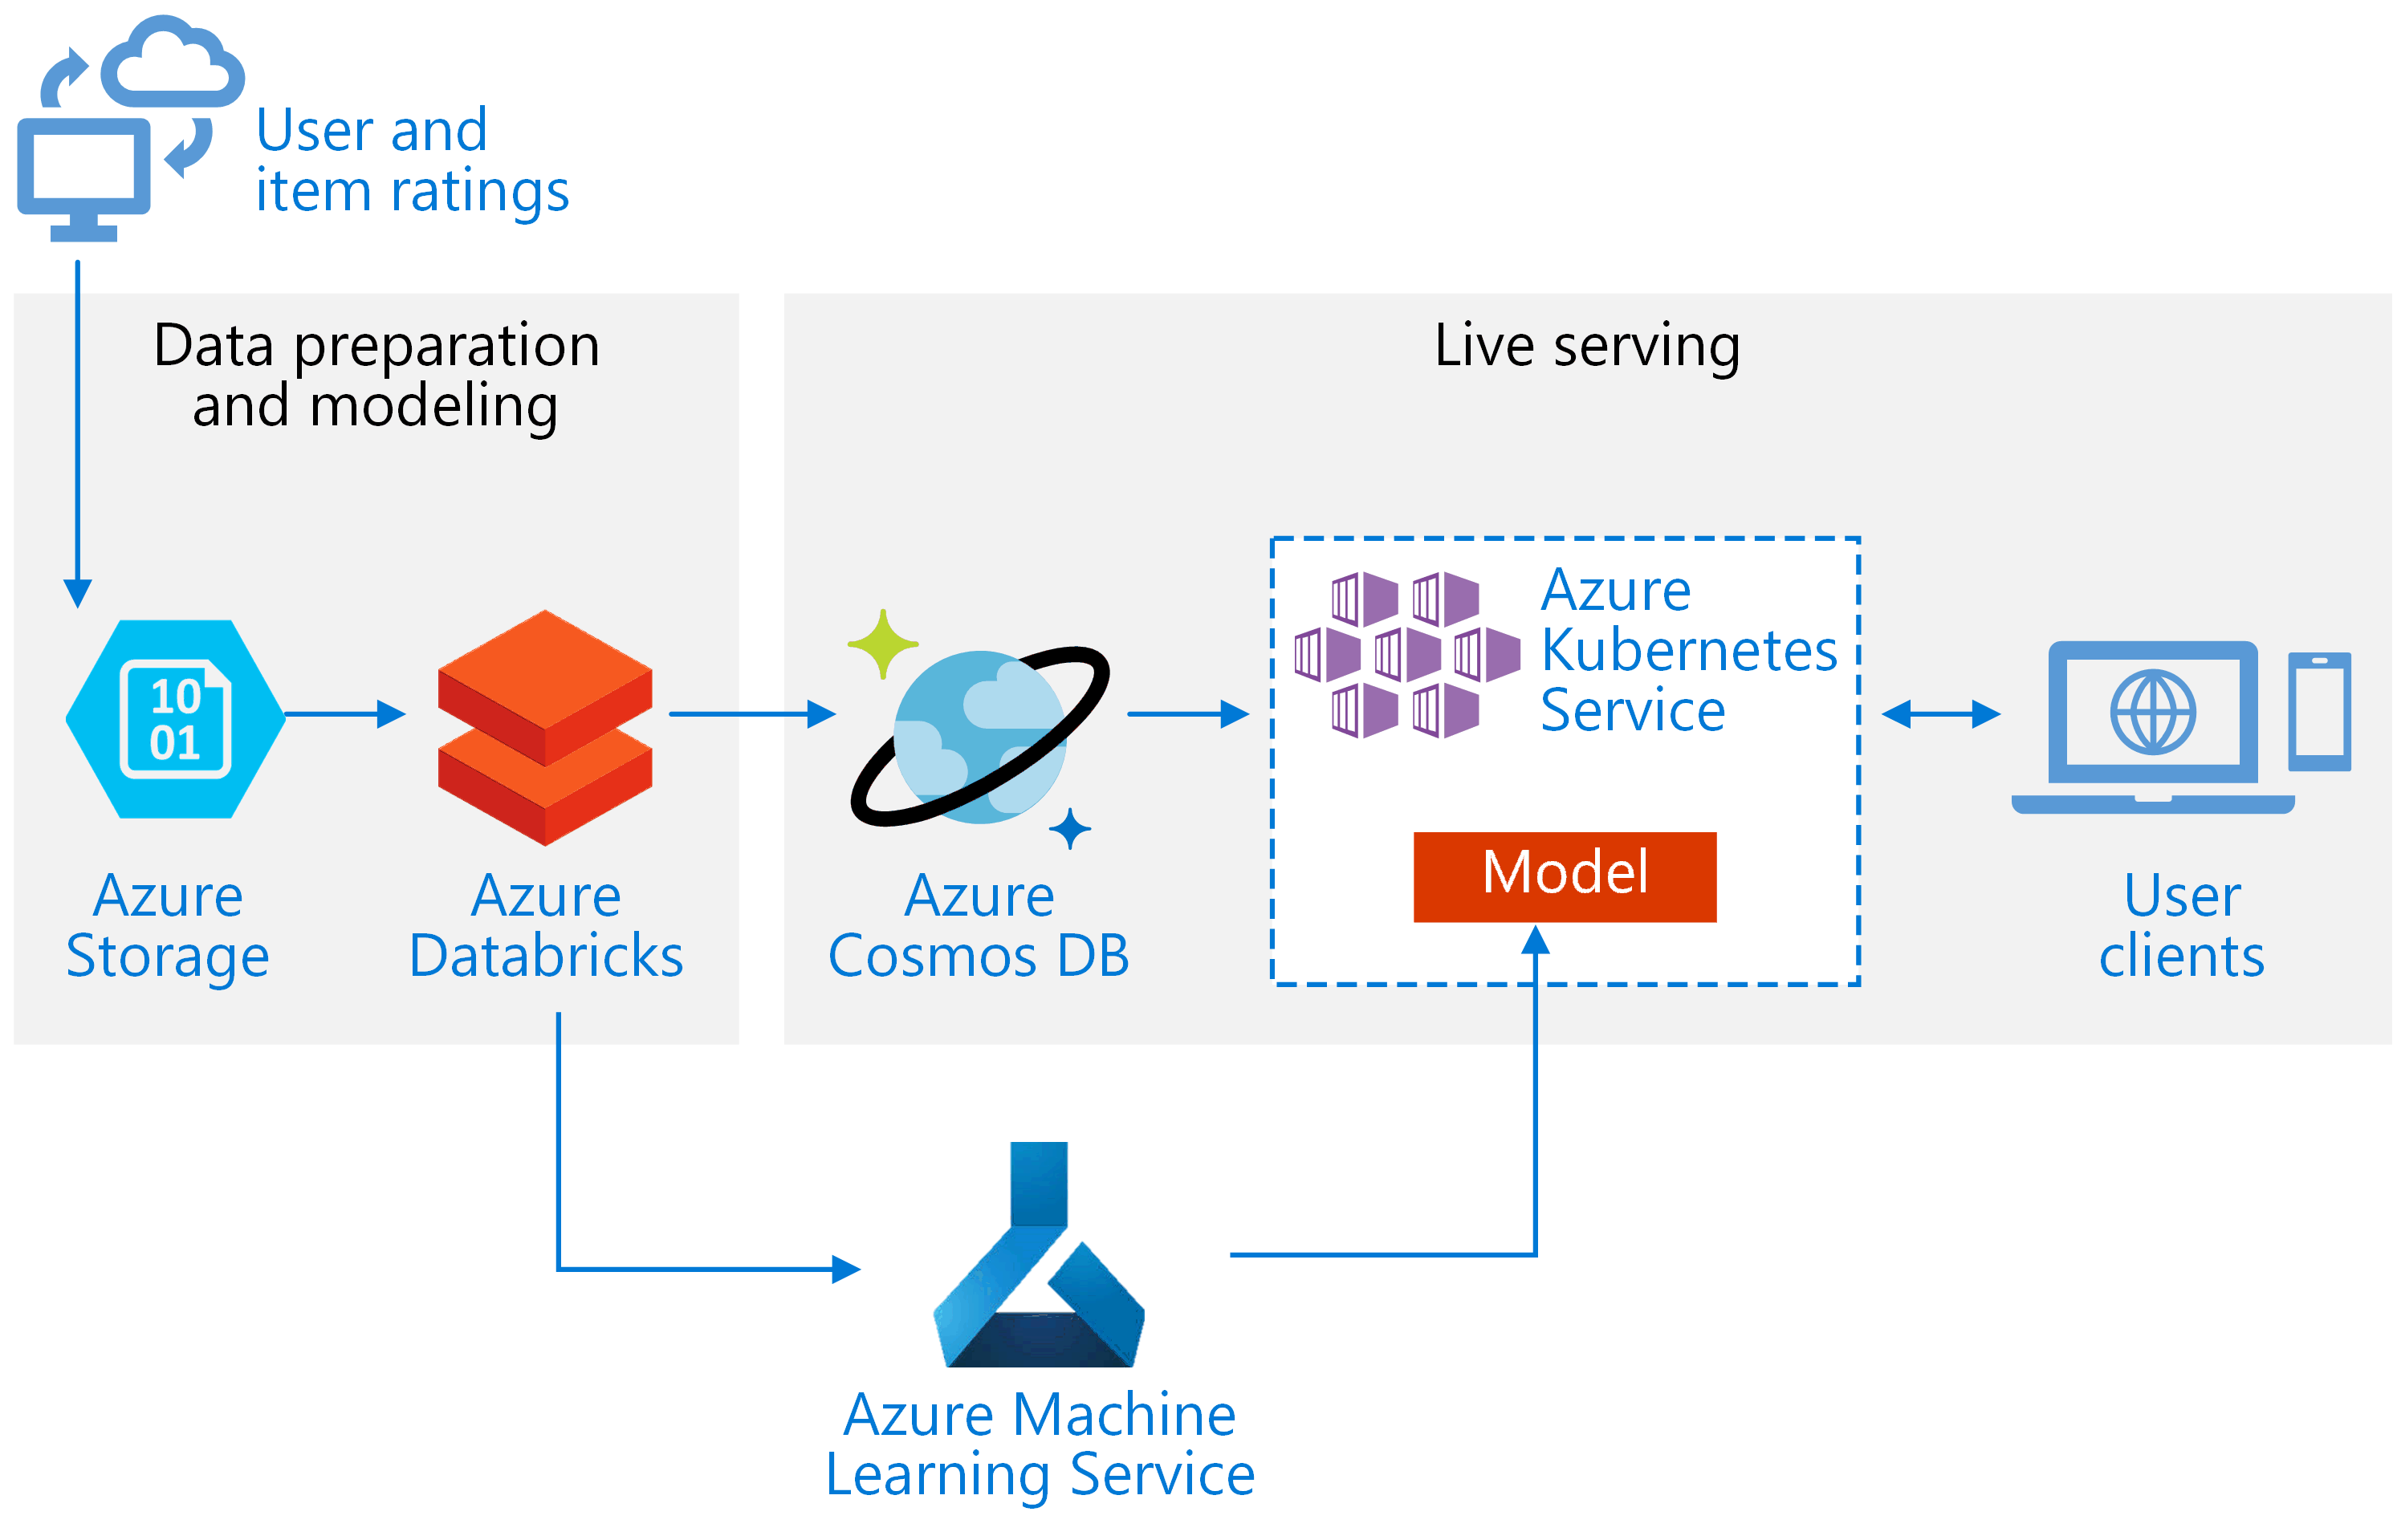
\includegraphics[width=0.8\textwidth]{figures/chapter_classification/azure_ml.png}
\caption{The architecture of Azure Machine Learning Service}
\label{fig.azure_ml}
\end{figure}

This paper aims to investigate if black-box adversarial attacks have become a practical threat against image classification cloud services. Our research majorly focuses on gradient estimation and local search via queries, and we use distributed black-box attacks to accelerate the time-consuming query process. Our main contributions are as follows: 

\begin{itemize}
    \item We identify some common mistakes in prior research that have led to an overestimation of the efficiency of black-box attacks (see Fig. \ref{fig:local}). To avoid these mistakes, we design an image classification cloud service for our experiments, and we open-source this cloud API for future research on black-box attacks\footnote{The source code of 
    DeepAPI is available on Github: \url{https://github.com/wuhanstudio/deepapi}.} (see Fig. \ref{fig:cloudapi}).
    \item We design a framework that facilitates horizontally and vertically distributed queries to speed up online black-box attacks against cloud services\footnote{The source code of the online black-box attacks is available on Github: \url{https://github.com/wuhanstudio/adversarial-classification}.} (see Fig. \ref{fig:distributability}). 
    \item We also provide an open-source black-box adversarial toolbox that simplifies the process of conducting black-box attacks against cloud APIs\footnote{The source code of the black-box adversarial toolbox is available on Github: \url{https://github.com/wuhanstudio/blackbox-adversarial-toolbox}.}. 
\end{itemize}

\begin{figure*}[btph]
    \centering
    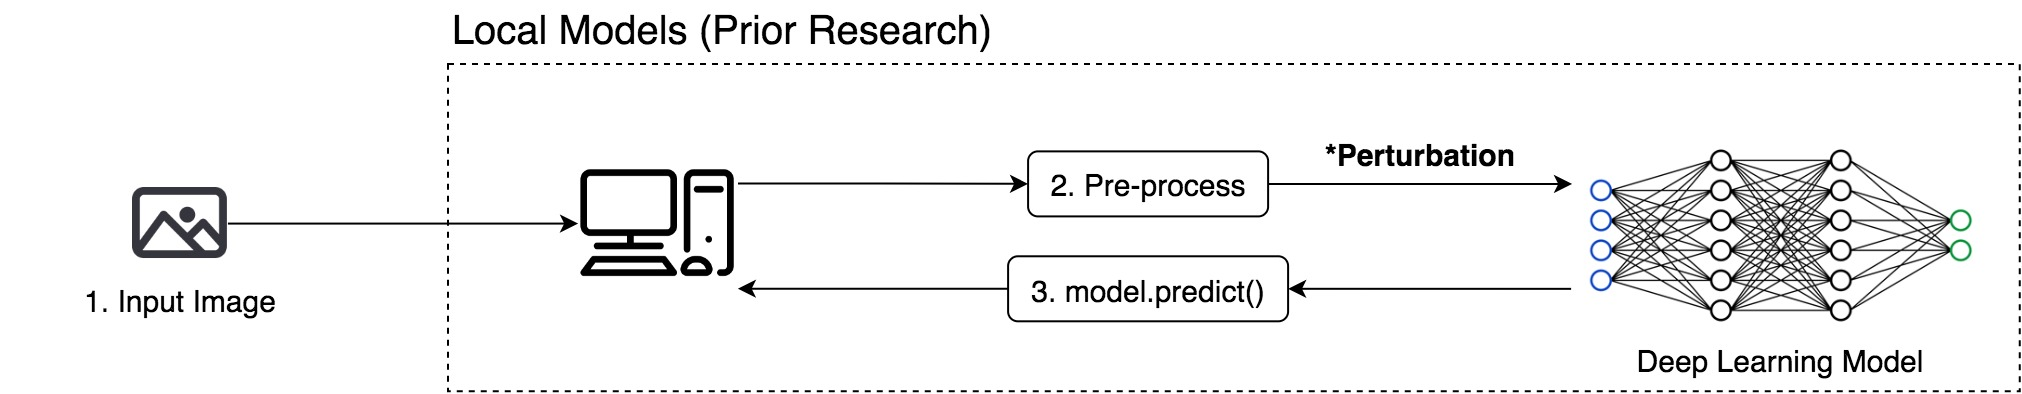
\includegraphics[width=0.9\linewidth]{figures/chapter_classification/local.jpg}
    \caption{Most prior research used local models to test black-box attacks.}
    \label{fig:local}
\end{figure*}

\begin{figure*}[btph]
    \centering
    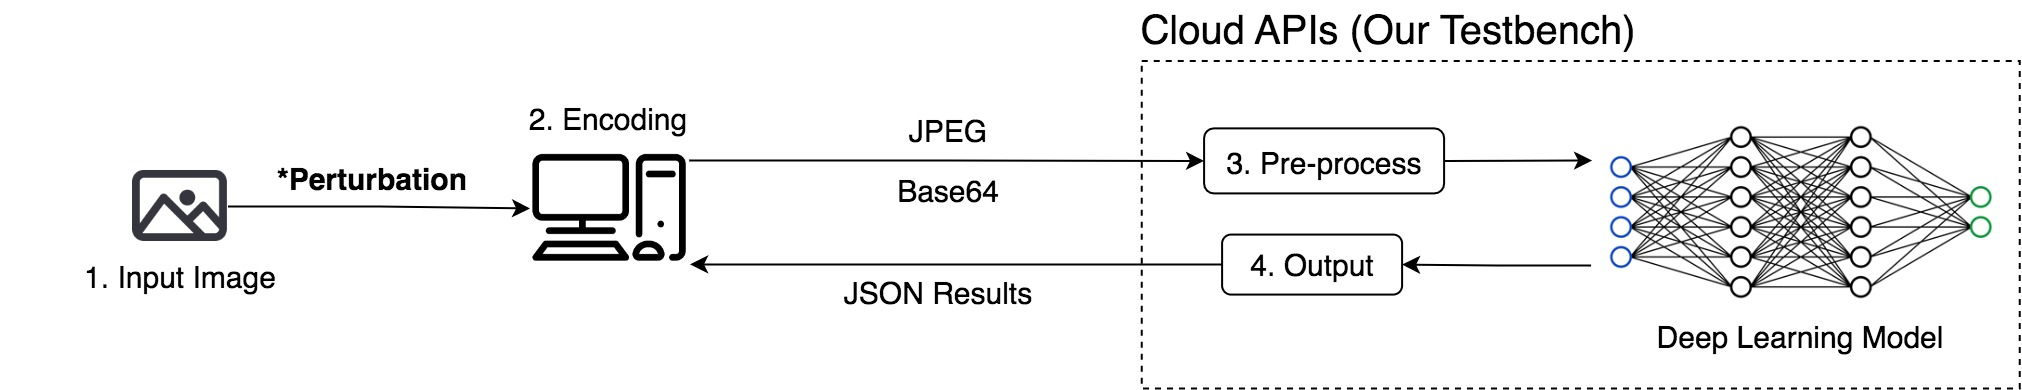
\includegraphics[width=0.9\linewidth]{figures/chapter_classification/cloudapi.jpg}
    \caption{We initiate the black-box attacks directly against cloud services.}
    \label{fig:cloudapi}
\end{figure*}

\begin{figure*}[btph]
    \centering
    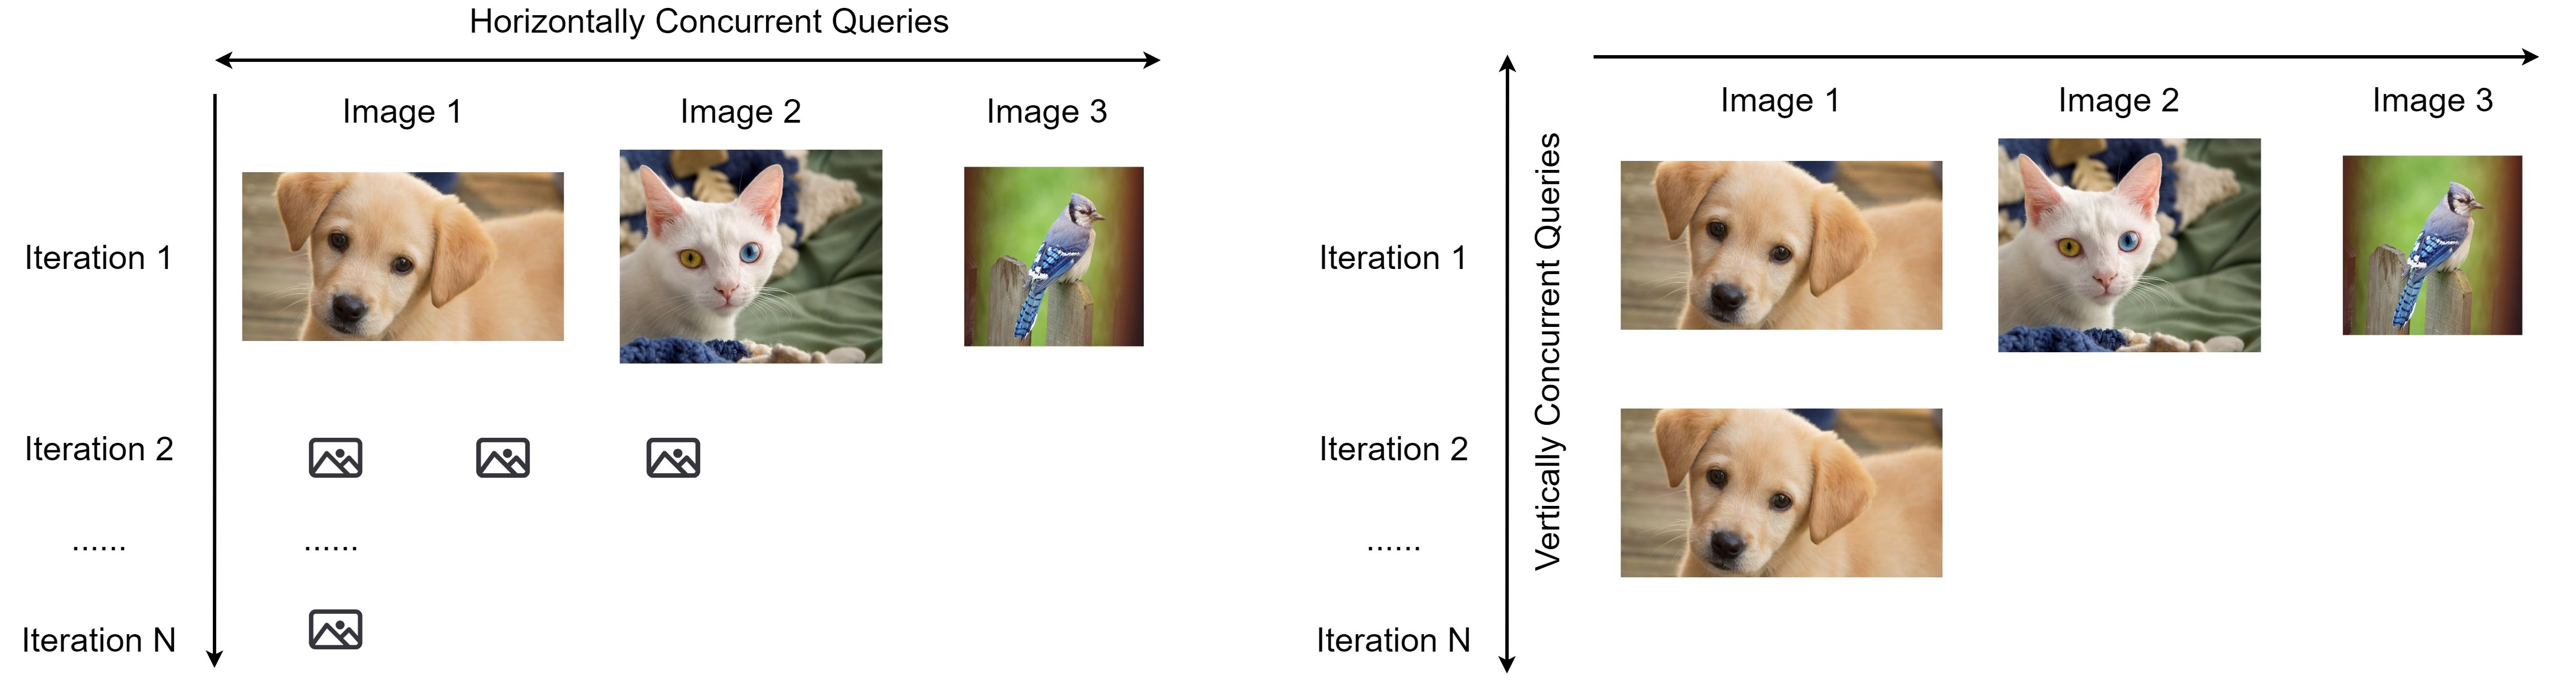
\includegraphics[width=0.9\linewidth]{figures/chapter_classification/distribution.jpg}
    \caption{The difference between horizontal and vertical distribution.}
    \label{fig:distributability}
\end{figure*}

\subsection{Common Mistakes}
\label{common_errors}

% \subsubsection{Attacking Cloud Services}

During our implementation of distributed black-box attacks, we observed that some previous research made certain errors in the query process, which provided their attacks with an unfair advantage. This advantage led these methods to outperform state-of-the-art black-box attacks, but it was based on the assumption of accessing information that is not available in black-box attacks \citep{ilyas2018black}\citep{ilyas2018prior}\citep{guo2019simple}\citep{Brunner_2019}\citep{moon2019parsimonious}\citep{andriushchenko2020square}.

\textbf{Image Encoding}: In real-world scenarios, images are typically encoded before being sent to image classification cloud services to reduce the amount of data transmitted and to save bandwidth (see Fig. \ref{fig:cloudapi}). However, prior research often assumes that perturbations can be added directly to the raw input image (see Fig. \ref{fig:local}). 

It is worth noting that cloud services such as Google Cloud Vision and Imagga accept raw binary and base64 encoded JPEG (lossy compression) images as input. This compression may cause some of the perturbations to disappear, ultimately reducing the success rate of attacks. Therefore, if we evaluate black-box attacks on local models without considering image encoding and quantization, we may overestimate the effectiveness of these attacks against real-world cloud APIs.

Besides, image classification cloud services do not accept images with invalid pixel values. For example, the bandit attack does not clip the image while estimating gradients, assuming they can send invalid images (pixel value $>$ 255 or $<$ 0) to the black-box model.

\textbf{Image Pre-processing}: Some papers apply perturbations \emph{after} image resizing, thereby assuming that they know the input shape of the image classification model in the cloud. Moreover, note that original input images are typically larger than the model input shape. Resizing high-resolution images to a lower resolution reduces the sampling space, thereby making it less computationally intensive to generate perturbations. 

Most prior research test their attacks on local models, rather than on online models, since it is both faster and less costly. Our experimental results reveal that these attacks achieve significantly lower success rates when attacking cloud services.

\subsection{Possible Causes}

Most prior research test their attacks on local models, rather than on online models, since it is both faster and less costly.  
%It could take 0.5-1.0 seconds to receive a single query result from an API server. On the other hand, querying local models on a computer can achieve over 100 queries per second with a GPU. Besides, 

Sending queries to real-world cloud APIs typically costs around \$1 for every 1,000 requests (for example, using Google Cloud Vision). In other words, an experiment attacking 1,000 images may require over 500,000 queries and cost more than \$500. Thus, most prior research tested their attacks on local models and relied on themselves to restrain access to extra model information. However, intentionally or unintentionally, they may exploit extra information that improves their attacks due to the following reasons:

\begin{itemize}
    \item The prediction function accepts raw images as float numbers and will not give an error even if the input image $x$ contains negative values. Thus, prior research did not encode input images and was unaware of that they might send invalid images to the model.
    \item The prediction function only accepts input images $x$ as an array. Thus, it is tempting to resize all input images to be the input size, thereby exploiting extra information about the model input shape.
\end{itemize}

% As a result, some prior research compared their methods with others on local models with unfair settings. 

In the next section, we introduce our open-source image classification cloud service. This cloud service will both facilitate future research and prevent these mistakes so that we can obtain a fair comparison of existing black-box attacks.

\section{Preliminaries}

\subsection{Image Classification Models}

Image classification models assign each image with pre-defined labels. The State-Of-The-Art models that use convolutional neural networks achieve more than 90\% Top-1 accuracy on the ImageNet dataset. The most popular models among them are ResNet, MobileNet, InceptionV3, and EfficientNet, because they achieve a good balance between model size and accuracy. It is of great importance to investigate the robustness of these models so that they can be securely deployed in cloud services. 

For adversarial attacks against image classification APIs, the adversary have no access to the models behind the infrastructure. Thus they can only query using black-box adversarial attacks. Prior research usually use ResNet-50 \citep{he2016deep}, VGG-16 \citep{simonyan2014very} and Inception-V3 \citep{szegedy2016rethinking} to test their attacks.

\begin{figure}[H]
\centering
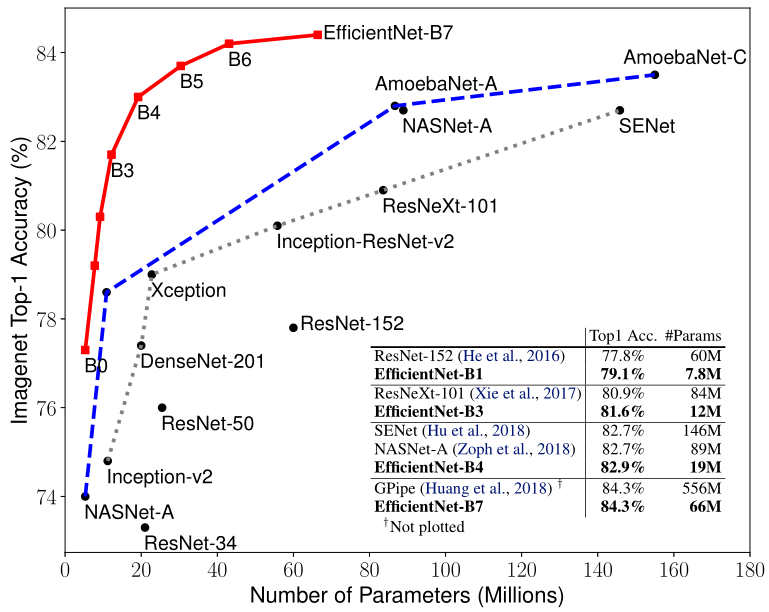
\includegraphics[scale=0.55]{figures/chapter_classification/efficient_net.png}
\caption{Model Size vs. ImageNet Accuracy \citep{tan2019efficientnet}}
\label{fig.efficient_net}
\end{figure}

The VGGNet is well known for its simplicity. A sequential of 3x3 convolutional layers and max-pooling layer are stacked on each other, followed by three fully-connected layers. When VGG was introduced in 2014, VGG-16 and VGG-19 are considered relatively deep. Now, we have more computational resources for much deeper architecture.

\begin{figure}[H]
\centering
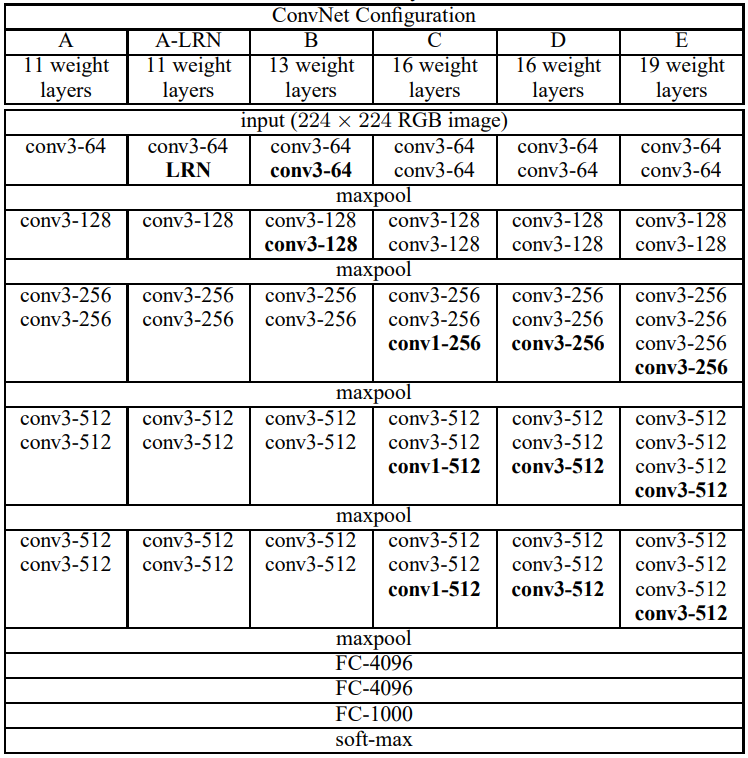
\includegraphics[scale=0.5]{figures/chapter_classification/vggnet.png}
\caption{VGGNet configurations}
\label{fig.vgg_net}
\end{figure}

In 2015, ResNet makes it possible to train up to hundreds or even thousands of layers. The residual building block introduces skip connections to solve the problem of vanishing gradient in deep CNNs while keeping the overall performance. Though we can train relatively deep ResNet, ResNet-50 and ResNet-101 are most widely used for image classification tasks because a deeper neural network requires more computational resources as well. It's unnecessary to increase the number of parameters if the accuracy satisfies our requirements.

\begin{figure}[H]
\centering
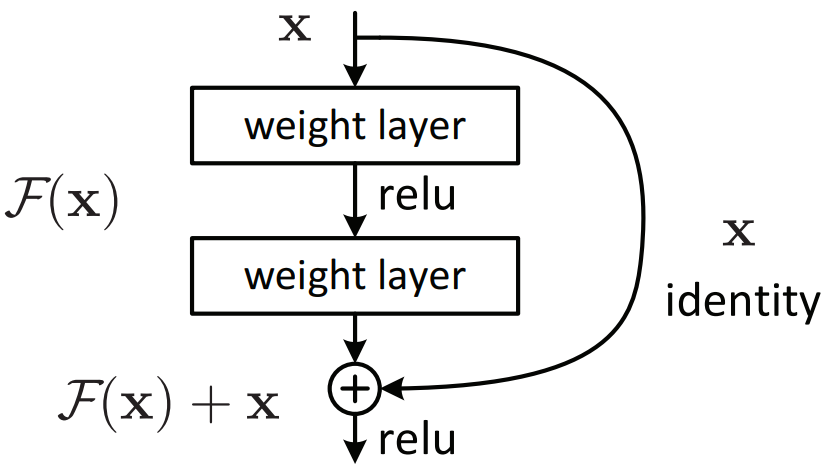
\includegraphics[scale=0.35]{figures/chapter_classification/resnet.png}
\caption{The residual building block}
\label{fig.res_net}
\end{figure}

The inception module was introduced by Google, and thus the first version is also known as GoogleNet. The choice of kernel size for convolution layers is tricky. Introducing different kernel sizes in different layers requires more computational resources and could suffer from the vanishing gradient problem. The inception module puts several convolution layers with different kernel sizes side-by-side at the same level, and extra 1x1 convolutions are introduced to control the number of features. Besides, an auxiliary is added to the original loss to avoid the vanishing gradient problem.

\begin{figure}[H]
\centering
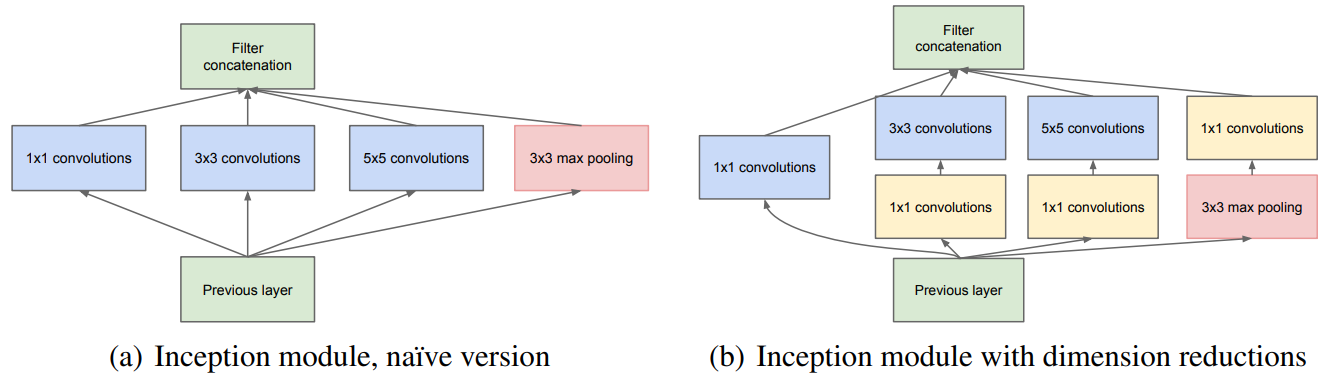
\includegraphics[width=0.9\textwidth]{figures/chapter_classification/inception.png}
\caption{The inception module}
\label{fig.inception}
\end{figure}

However, all of the three models are vulnerable to adversarial attacks. It is possible to generate adversarial examples via querying the model.

\subsection{Black-box Adversarial Attacks}
\label{black_box}

Black-box adversarial attacks aim to fool deep learning models without access to the models' structure and weights. Besides, the perturbation for a successful attack should be unnoticeable by human eyes, which is usually measured by the $L_p$ norm. Current black-box adversarial attacks can be classified into four categories: gradient estimation, transferability, local search, and combinatorics \citep{bhambri2019survey}.

\begin{figure}[H]
\centering
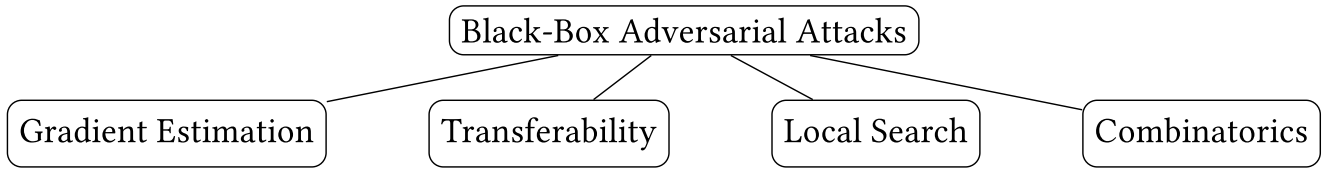
\includegraphics[width=0.9\textwidth]{figures/chapter_classification/review.png}
\caption{Classification of prior work on black-box scenario-based attacks \citep{bhambri2019survey}}
\label{fig.bb_review}
\end{figure}

\textbf{Gradient Estimation}: The idea of gradient-based methods is inspired by white-box adversarial attacks. White-box attacks rely on gradients to generate adversarial perturbations. Under the scenario of a black-box attack, we do not have access to gradients. Thus we may approximate gradients through queries, and then use estimated gradients to generate perturbations. 

\textbf{Transferability}: Also, We can generate adversarial perturbations by taking advantage of transferability. The targeted deep learning model is the oracle. Through querying the oracle model, we can construct a synthetic dataset. The attacker uses the synthetic dataset to train a surrogate model. Adversarial inputs generated using the surrogate model could fool the oracle model due to the characteristic of transferability.

\textbf{Local Search}: Additionally, we can treat the problem of generating adversarial inputs as selecting pixels to attack. Thus we can use existing local search methods to search for combinations of pixels to be attacked.  

\textbf{Combinatorics}: \citep{moon2019parsimonious} first reformulates the problem to be a linear program and finds the solution of the problem at the vertex of the $l_\infty$ ball. This method reformulates the problem from a new perspective, still we can  use existing local search methods to solve the reformulated problem.

All methods require querying the target model. For adversarial attacks against cloud services, there is an additional constraint on the number of queries. The number of queries required for a successful attack is critical because cloud platforms charge per API call. The more you query, the more it costs for every single attack. Thus, we focus on methods that require fewer queries.

\begin{figure}[H]
\centering
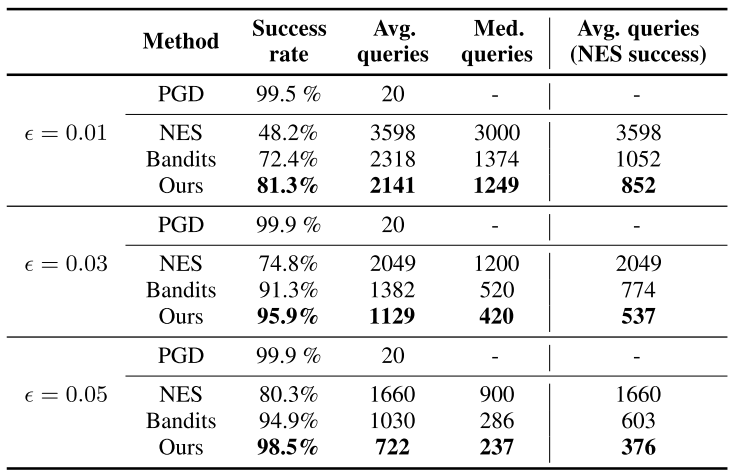
\includegraphics[scale=0.65]{figures/chapter_classification/parsimounious.png}
\caption{Results for $l_{\infty}$ untargeted attacks on ImageNet \citep{moon2019parsimonious}}
\label{fig.parsi}
\end{figure}

One simple yet effective method is the Simple Black-box Attack (SimBA) \citep{guo2019simple}. We can randomly sample a vector from a predefined orthonormal basis and either add or subtract it to gradually deviate the classification results. However, this method is less effective if the perturbation added to each pixel is smaller than 0.4, making this attack more conspicuous. Another more sophisticated method proposed by Andrew Ilyas, etc \citep{ilyas2018black} estimates the gradient using the Natural Evolutionary Strategies (NES). Since then, evolutionary strategies have been widely adopted in the scenario of black-box adversarial attacks as in \citep{meunier2019yet} \citep{Ilie2021}.

\begin{figure}[H]
\centering
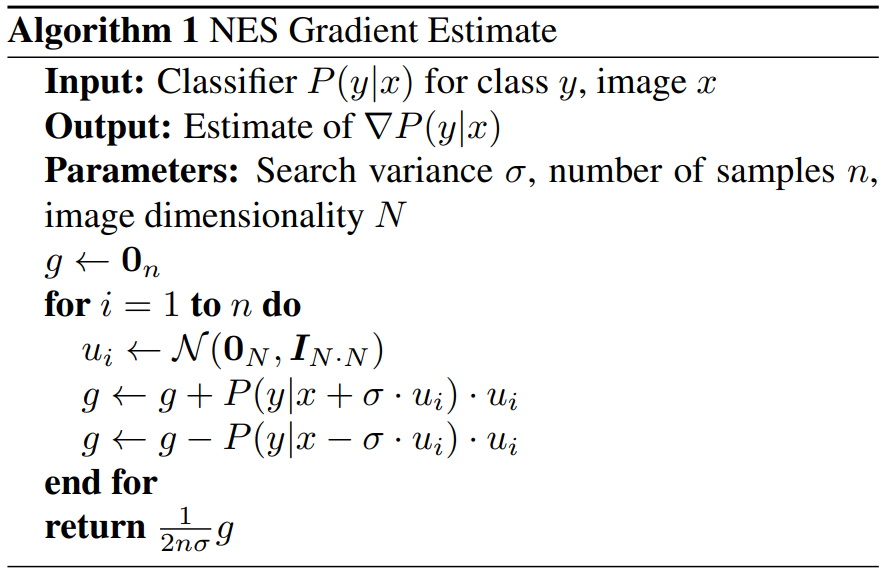
\includegraphics[scale=0.55]{figures/chapter_classification/nes.png}
\caption{The Natural Evolutionary Strategies for gradient estimation.}
\label{fig.nes}
\end{figure}

\section{Distributed Black-box Attacks}

% \subsection{Problem Formulation}

% Given some input image $x$ and true labels $y$, the objective of the adversary is to add a small perturbation $\delta$ to the original image, and generate an adversarial image $x' = x\ +\ \delta$ that can fool a black-box image classifier $C(x)$, such that $C(x') \neq C(x)$. Typically, the perturbation $\delta$ is bounded in the $l_2$ or $l_\infty$ norm by some user-defined constant \citep{bhambri2019survey}.

% The adversary does not know the model structure and weights. Further, the attacker has limited access to model outputs for black-box models deployed on cloud servers. For example, in the partial-information setting, the adversary only has access to the prediction probabilities of the top $k$ classes $\{y_1, ..., y_k\}$. In the label-only setting, the adversary can only access the prediction label without any knowledge of prediction probabilities \citep{ilyas2018black}.

\subsection{Distributed Queries}

Cloud computing platforms serve APIs via load balancing, which means that several computing engines provide the same model-inference service simultaneously. If we exploit load balancing and send multiple queries concurrently, we can receive all the results simultaneously and thus accelerate black-box attacks significantly. 

To demonstrated this hypothesis, we sent 1, 2, 10, and 20 queries concurrently to Google Cloud Vision, Imagga, and DeepAPI. Since the PC has eight cores, we sent concurrent queries from eight workers. Tab. \ref{table_query} lists the total time, averaged over 10 experiments, before receiving all responses. As can be seen, the total time does not grow linearly with the number of queries. Rather, the average query time decreases as we send out more concurrent queries.

% Black-box attacks are usually slow because they require several thousands of queries. Depending on the network quality, it could take 0.5$-$2s to receive one query result from an API server, and thus, it could take several hours to launch a black-box attack. However, cloud computing platforms serve APIs via load balancing, which means that several computing engines provide the same model-inference service simultaneously. If we exploit load balancing and send multiple queries concurrently, we can receive all the results simultaneously and thus accelerate black-box attacks significantly. 

\begin{table}[tbph]
\begin{center}
\begin{tabular}{ccacaca}
    \hline
    Queries       & \multicolumn{2}{c}{Cloud Vision} & \multicolumn{2}{c}{Imagga}      & \multicolumn{2}{c}{DeepAPI} \\
    \hline
    & Total  & Average & Total & Average & Total  & Average \\
    \hline
    1       & 446.7ms  & 446.7ms & 1688.1ms & 1688.1ms & 538.5ms  & 538.5ms \\
    2      & 353.61ms  & 176.8ms & 2331.81ms & 1165.9ms  & 643.2ms  & 321.6ms  \\
    10    & 684.25 ms & 68.4ms  & 10775.8ms & 1077.6ms & 1777.8ms & 177.8ms  \\
    20    & 1124.82ms & 56.2ms & 21971.8ms & 1098.6ms & 1686.4ms & 84.3ms \\
    \hline
\end{tabular}
\end{center}
\caption{The total and average time of sending concurrent queries to cloud APIs.}
\label{table_query}
\end{table}

% \begin{figure}[btph]
%     \centering
%     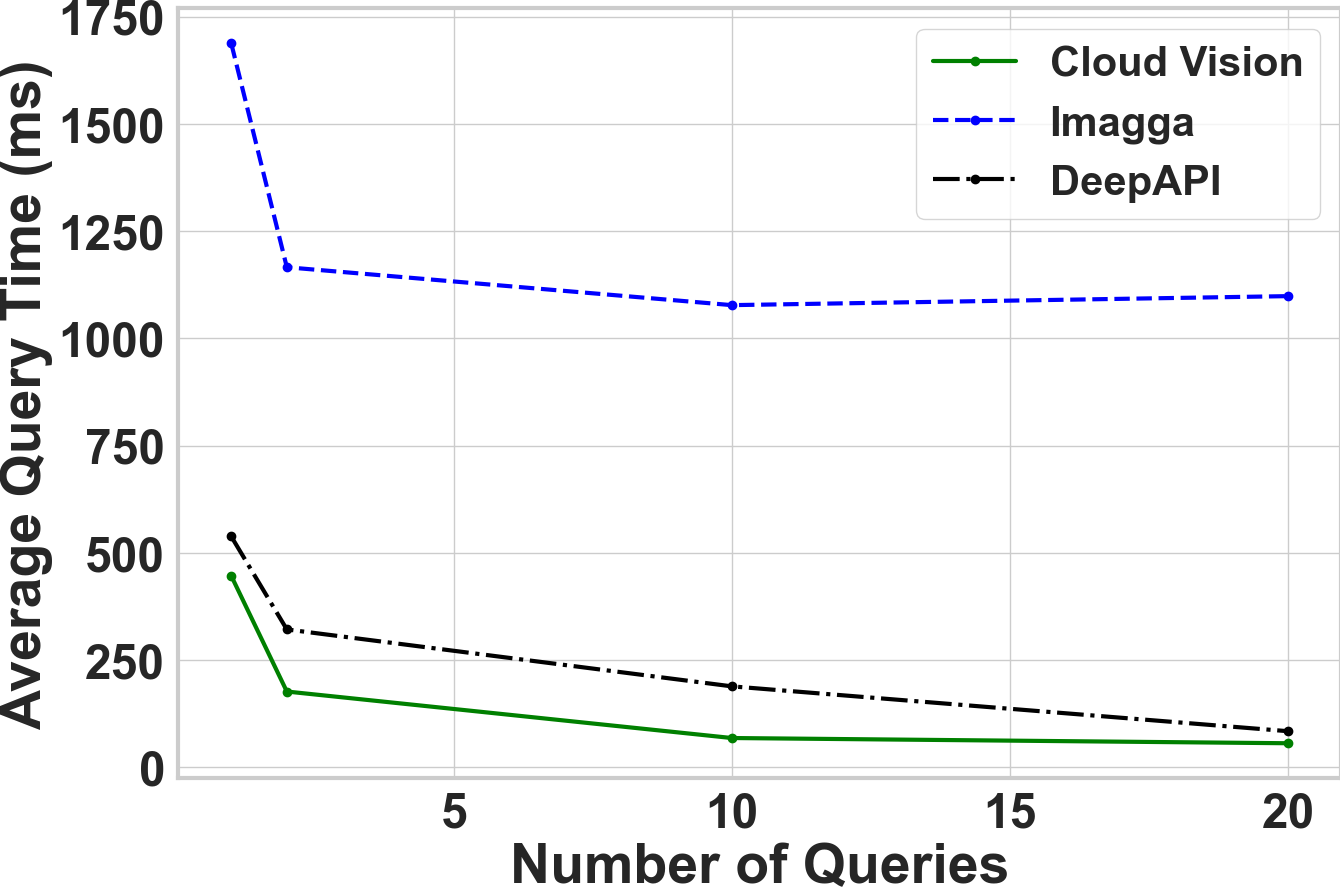
\includegraphics[width=0.5\textwidth]{figures/chapter_classification/average_query_time.png}
%     \caption{The average query time when sending multiple concurrent queries to cloud APIs.}
%     \label{fig:dist_query}
% \end{figure}

% In conclusion, thanks to load balancing, the more queries we send, the faster the queries become on average. This is a feature that we will exploit to accelerate black-box attacks. 

% \clearpage

% \subsubsection{DeepAPI}

% To facilitate future research on distributed black-box attacks that attack cloud APIs rather than local models, we designed DeepAPI, an open-source image classification cloud service (see Fig. \ref{fig:deepapi}) that supports:

% \begin{itemize}
%     \item The three most popular classification models for black-box attacks: VGG16, ResNet50, and Inceptionv3 provided by Keras Model Zoo \citep{chollet2015keras}.
%     \item Both soft labels (with probabilities) and hard labels (without probabilities) for label-only setting.
%     \item Top $k$ predictions ($k \in \{1, 3, 5, 10\}$) for partial-information setting.
%     % \item Web UI and distributed API requests.
% \end{itemize}

% \begin{figure*}[btph]
%     \centering
%     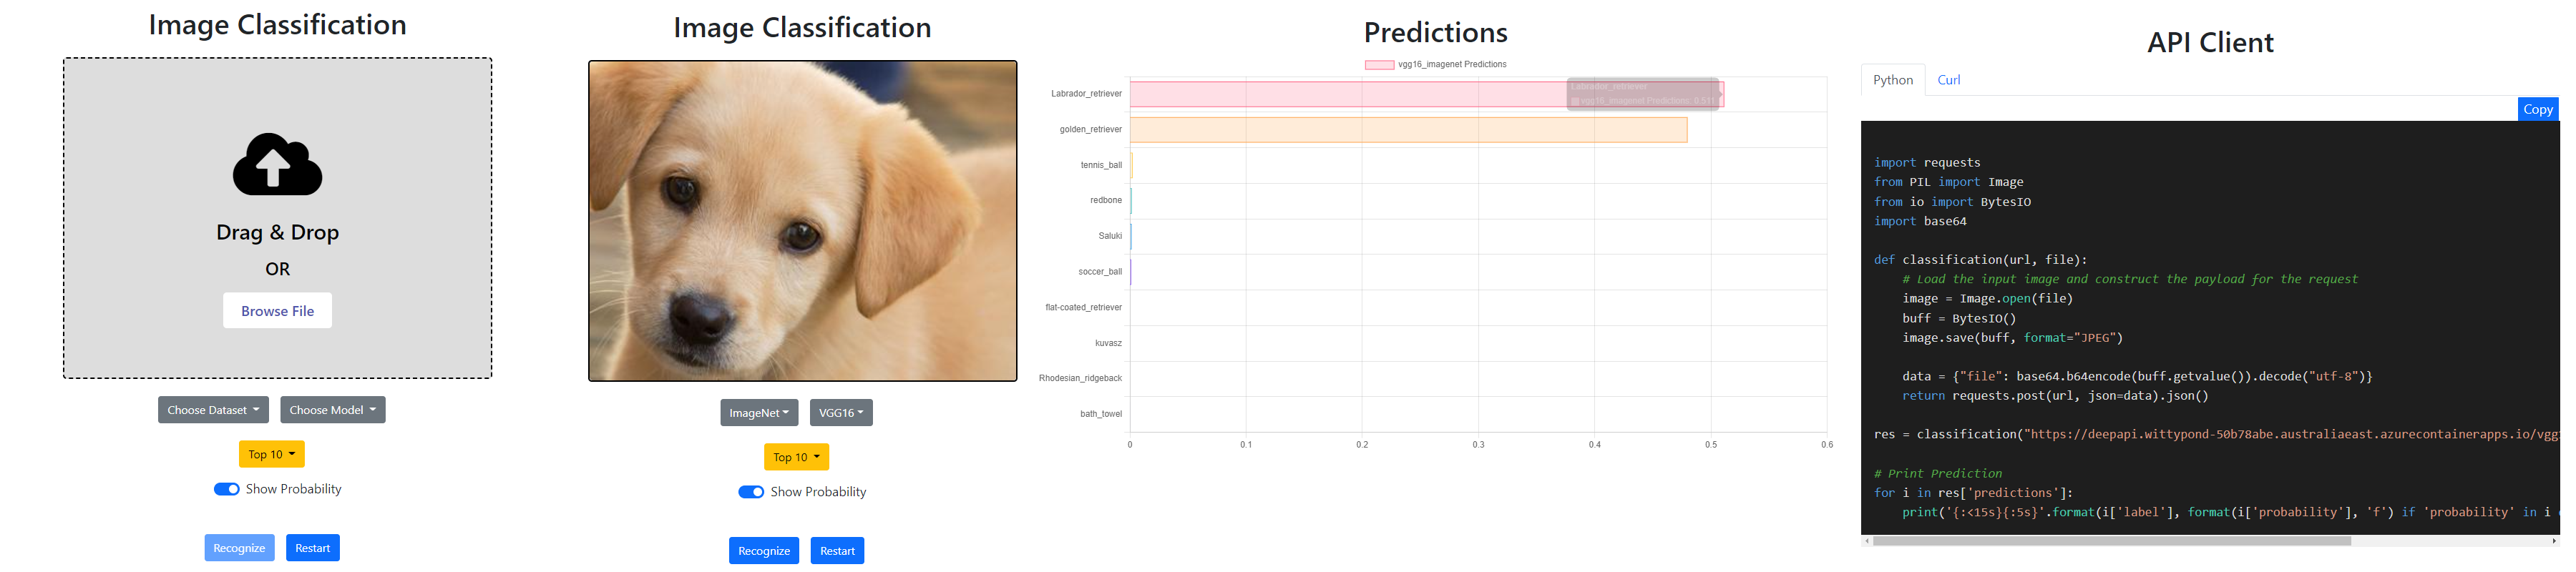
\includegraphics[width=\linewidth]{figures/chapter_classification/deepapi.png}
%     \caption{DeepAPI provides both web interface and APIs for research on black-box attacks.}
%     \label{fig:deepapi}
% \end{figure*}

% \clearpage

\subsection{Horizontal and Vertical Distribution}
\label{horizon_vertical}

Both local (multi-core CPU) and cloud-based (load balancer) deep learning models are vulnerable to distributed queries, but the challenge lies in deciding which queries to send concurrently. To address this problem, we propose horizontal and vertical distribution for black-box attacks, inspired by horizontal and vertical scaling of cloud resources \citep{Millnert2020}.

Horizontal distribution concurrently sends queries for different images within the same iteration, thereby allowing the generation of multiple adversarial examples concurrently. This can be achieved without altering existing black-box attack methods. 

Vertical distribution, on the other hand, sends multiple concurrent queries for the same image, thereby accelerating the attack for that particular image. Existing black-box attack methods need to be redesigned to decouple the queries across iterations.

In summary, horizontal distribution achieves concurrent attacks against multiple images, while vertical distribution speeds up attacks on a single image (see Fig. \ref{fig:distributability}). Since horizontal distribution does not require significant modifications to the original attack method, we can apply horizontal distribution by implementing a distributed query function that sends concurrent requests to cloud APIs. In the following sections, we focus on vertical distribution.


\subsubsection{Vertically Distributed SimBA and Square Attack (Local Search)}

We use the SimBA (baseline) \citep{guo2019simple} and the Square Attack \citep{andriushchenko2020square} to illustrate how to apply vertical distribution to local search methods. The problem formulation and original SimBA and Square Attack are illustrated in Section \ref{black_box}.

\textbf{The SimBA Attack}: To apply vertical distribution to SimBA, we need to decouple the correlation between queries at different iterations. The original SimBA attack can only choose which pixel to perturb after receiving previous query results and deciding the perturbation $\delta \in \{-\boldsymbol{q}\epsilon, +\boldsymbol{q}\epsilon\}$, where $\epsilon$ is the strength of the attack and $\boldsymbol{q}$ is the perturbation vector that decides the index of the perturbed pixel. Therefore, we send out queries for several $\boldsymbol{q}$ as a batch $\boldsymbol{q}_{batch}$ concurrently. The sign of each perturbation vector is decided independently to reduce the output probability of the highest class. Then, we sum and project the accumulated perturbation $\delta$ to the $L_2$ ball at the end of each iteration to guarantee imperceptibility.

% To decouple the correlation between queries at different iterations in SimBA, we devise a vertically distributed SimBA. This method generates a batch of perturbation vectors $\boldsymbol{q}_{batch}$ and sends out queries concurrently for each vector. The sign of each perturbation vector is decided independently, and the accumulated perturbation $\delta$ is updated after each batch of queries. To ensure imperceptibility, the accumulated perturbation is projected to the $L_2$ ball at the end of each iteration.

\textbf{The Square Attack}: To apply vertical distribution to the Square Attack, we generate a batch of square-shaped perturbations independently and send out queries concurrently for each perturbation. After receiving the queries, we add the perturbations that reduce the margin loss $l=L(C(X), y)=C_y(X)-\max_{k \neq y}C_k(X)$ to the image, where $y$ is the correct class of the input image X and $C_y(X)$ is the output probability of class $y$. Then, we project the accumulated perturbation to the $L_\infty$ ball to ensure imperceptibility (see Alg. \ref{alg:square_vertical}).

% $$L(C(X), y)=C_y(X)-max_{k \neq y}C_K(X)$$

% The Square Attack is a local search method, just like SimBA. However, it is generally more query-efficient. As its name suggests, the square attack generates square-shaped perturbations to decrease the margin loss $L(C(X^{'}, y))$. The square attack improves query efficiency by initializing the perturbation with vertical stripes, motivated by the fact that CNNs are sensitive to high-frequency perturbations \citep{yin2019fourier}. We apply horizontal distribution to both the initialization and iteration processes across images.

% \subsection{Distributed SimBA (Baseline Method)}

% In each iteration, SimBA increases or decreases the value of one randomly chosen pixel, and assumes that for any perturbation vector $\boldsymbol{q}$ and some step size $\epsilon$, either $x + \epsilon\boldsymbol{q}$ or $x - \epsilon\boldsymbol{q}$ will decrease the highest probability $p_h(x')$ in $y = (p_1, p_2, ..., p_K)$. Thus, we can randomly pick a vector $\boldsymbol{q}$ in the set of orthogonal search directions $Q$ and then either add or subtract it from the image $x$ to decrease the highest probability $p_h(x')$. To guarantee maximum query efficiency, $\boldsymbol{q}$ are picked from $Q$ without replacement, and all vectors in $Q$ are orthonormal. More details can be found in the documentation of the toolbox.

% The distributed SimBA is not only faster but also generates less perceivable perturbations. The original SimBA manipulates one pixel each time at a small step $\epsilon$, while the distributed version modifies multiple pixels and the sum of them is bounded by $\epsilon$. Thus, the distributed SimBA modifies each pixel at a smaller step than the original SimBA.

\subsubsection{Vertically Distributed Bandits Attack (Gradient Estimation)}

The Bandits Attack is a gradient estimation method that improves the optimal least-squares estimator by introducing gradient priors \citep{ilyas2018prior}. The perturbation vector $q_i=v_i+\delta u_i$ is computed from the gradient prior $v_i$ and a Gaussian vector $u_i$ sampled from $\mathcal{N}(0, \frac{1}{d_i}I)$. 

The Bandits Attack uses imperfect gradient estimators $\nabla_i= \frac{l(v_i+\delta u_i)-l(v_i-\delta u_i)}{\delta} u_i$ to improve query efficiency at the cost of introducing noises in the estimations. Therefore, averaging over a batch of concurrent gradient estimations can improve the accuracy and efficiency. In addition, adversarial images $x'$ are updated using projected gradient descent (PGD), while gradient priors are updated using exponentiated gradients (EG) \citep{pmlr-v117-ghai20a} (see Alg. \ref{alg:bandits_vertical}).

% The horizontally distributed Bandits Attack estimates gradients of different images simultaneously, while the vertically distributed Bandits Attack concurrently estimates a batch of gradients for the same image. 

% \clearpage

% \begin{minipage}{0.9\textwidth}
% \begin{algorithm}[H]
%     \centering
%     \caption{Horizontal Distribution}
%     \label{alg:horizontal}
%     \begin{algorithmic}
%         \STATE {\bf Input}: Input images $x \in X$, and the number of iterations $n_{iter}$ for each image.
%         \STATE {\bf Output}: Adversarial images $x' \in X'$. 
%         % \STATE
%         \STATE Initialize: $X^{'}$.
%         \FOR {each iteration $n \in [0,\ n_{iter})$}
%         \STATE //\ Concurrent requests across images.
%             \STATE $X^{'}$ = Black\_Box\_Attack$(X$, y)
%             \STATE \{
%             \begin{ALC@g}
%                 \STATE Update $X^{'}$.
%                 \STATE Concurrent Queries: y{'} = C($X{'}$).
%             \end{ALC@g}
%             \STATE \}
%             \STATE \textbf{if} {success rate == 100\%} \textbf{then} {\textbf{break}}.
%         \ENDFOR
%     \end{algorithmic}
% \end{algorithm}
% \end{minipage}

% % \clearpage

% \begin{minipage}{0.9\textwidth}
% \begin{algorithm}[H]
%     \centering
%     \caption{Vertical Distribution}
%     \label{alg:vertical}
%     \begin{algorithmic}
%         \STATE {\bf Input}: Input images $x \in X$, and the number of iterations $n_{iter}$ for each image.
%         \STATE {\bf Output}: Adversarial images $x' \in X'$.
%         % \STATE
%         \FOR {each image $x_{i} \in X$}
%             \STATE $x'_{i}$ = Black\_Box\_Attack($x_{i}$, $y_{i}$, batch)
%             \STATE \{
%             \begin{ALC@g}
%                 \STATE Initialize: $x'_{i}$.
%                 \STATE //\ Concurrent requests across iterations.
%                 \FOR {each iteration $n \in [0,\ n_{iter})$}
%                 \STATE Generate a batch of $X^{'}_{batch}$ based on $x'_i$.
%                 \STATE Concurrent Queries: $y'_{batch} = C(X^{'}_{batch}$).
%                 \STATE Update $x'_{i}$.
%                 \STATE $n = n + batch$
%                 \STATE \textbf{if} {success} \textbf{then} {\textbf{break}}.
%                 \ENDFOR
%             \end{ALC@g}
%             \STATE \}
%         \ENDFOR
%     \end{algorithmic}
% \end{algorithm}
% \end{minipage}

% \clearpage

% \pagebreak

% \begin{minipage}{\textwidth}
% \begin{algorithm}[H]
%     \centering
%     \caption{Distributed SimBA (Horizontal)}
%     \label{alg:simba_horizontal}
%     \begin{algorithmic}
%         \STATE Initialize: $X^{'} = X$.
%         \FOR {each iteration $n \in [0,\ n_{iter})$}
%             \STATE $X^{'}, y^{'}$ = SimBA($X^{'},\ y',\ Q,\ \alpha, \epsilon$)
%             \STATE \{
%             \begin{ALC@g}
%                 \STATE $\Delta = [\ ]$
%                 \FOR {each image $x_{i} \in X$}
%                     \STATE \text{Pick $\boldsymbol{q} \in Q$ randomly without replacement.}
%                     \STATE \text{Append $\epsilon \boldsymbol{q}$ to $\Delta$.}
%                 \ENDFOR
%                 % \STATE
%                 \STATE //\ Concurrent requests across images.
%                 \STATE $p^+ = C(X{'} + \Delta$).
%                 \STATE $p^- = C(X{'} - \Delta$).
%                 % \STATE
%                 \FOR {each image $x_{i} \in X$}
%                     \If {$p_{i}^+ < \boldsymbol{y}'_i$}
%                         \STATE \text{$x'_i = x'_i + \alpha \boldsymbol{q}_i$} 
%                     \ELSIF{$p_{i}^- < \boldsymbol{y}'_i$}
%                         \STATE \text{$x'_i = x'_i - \alpha \boldsymbol{q}_i$} 
%                     \ENDIF
%                     % \STATE Update $y_i^{'}$.
%                 \ENDFOR
%             \end{ALC@g}
%             \STATE \}
%             \STATE \textbf{if} {success rate == 100\%} \textbf{then} {\textbf{break}}.
%         \ENDFOR
%     \end{algorithmic}
% \end{algorithm}
% \end{minipage}

% \hfill \break

\begin{minipage}{0.9\textwidth}
\begin{algorithm}[H]
    \centering
    \caption{Distributed SimBA (Vertical)}
    \label{alg:simba_vertical}
    \begin{algorithmic}
        \FOR {each image $x_{i} \in X$}
            \STATE $x'_{i},\ y'_{i}$ = SimBA($x_{i}$, $y_{i}, Q, \alpha, \epsilon, n_{batch}$)
            % \STATE \{
            \begin{ALC@g}
                \STATE Initialize: $\delta_i = 0, x'_{i} = x_i + \delta_i$.
                \FOR {each iteration $n \in [0,\ n_{iter})$}
                    \STATE \text{Pick $\boldsymbol{q}_{batch} \in Q$ randomly without replacement.}
                    % \STATE
                    \STATE //\ Concurrent requests across iterations.
                    \STATE $p^+ = C(x{'} + \boldsymbol{q}_{batch}\epsilon$).
                    \STATE $p^- = C(x{'} - \boldsymbol{q}_{batch}\epsilon$).
                    % \STATE
                    \FOR{$\boldsymbol{q}_i \in \boldsymbol{q}_{batch}$}
                        \IF {$p_{i}^+ < \boldsymbol{y}'_i$}
                            \STATE \text{$\delta^{'}_i = \delta^{'}_i + \alpha \boldsymbol{q}_i$} 
                        \ELSIF{$p_{i}^- < \boldsymbol{y}'_i$}
                            \STATE \text{$\delta^{'}_i = \delta^{'}_i - \alpha \boldsymbol{q}_i$} 
                        \ENDIF
                    \ENDFOR
                    % \STATE
                    \STATE $\delta_i = proj_{p}(\delta_i)$
                    \STATE $x'_i = x'_i + \delta_i$
                    % \STATE Update $y_i^{'}$.
                    \STATE $n = n + n_{batch}$
                    \STATE \textbf{if} {success} \textbf{then} {\textbf{break}}.
                \ENDFOR
            \end{ALC@g}
            % \STATE \}
        \ENDFOR
    \end{algorithmic}
\end{algorithm}
\end{minipage}

% \clearpage

% \begin{minipage}{\textwidth}
% \begin{algorithm}[H]
%     \centering
%     \caption{Distributed Square Attack (Horizontal)}
%     \label{alg:square_horizontal}
%     \begin{algorithmic}
%         \FOR {each image $x_{i} \in X$}
%             \STATE Initialize: $x'_{i} = init(x_{i})$ with vertical strips.
%             \STATE //\ Concurrent requests across images.
%             \STATE $l^{*}_i = L(C(x'_i), y)$.
%         \ENDFOR
%         \FOR {each iteration $n \in [0,\ n_{iter})$}
%             \STATE $X^{'},\ y'$ = SquareAttack($X^{'},\ y', \epsilon$)
%             \STATE \{
%             \begin{ALC@g}
%                 \STATE $\Delta = []$
%                 \FOR {each image $x_{i} \in X$}
%                     \STATE $\delta_i =$ Uniformly sample a square perturbation.
%                     \STATE \text{Append $\delta_i$ to $\Delta$.}
%                 \ENDFOR
%                 \STATE //\ Concurrent requests across images.
%                 \STATE $l = L(C(X^{'} + \Delta), y')$.
%                 \FOR {each image $x_{i} \in X$}
%                     \If {$l_{i} < l^{*}_i$}
%                         \STATE $x'_i = x'_i + \delta_i$
%                         \STATE $x'_i = proj_{p}(x'_i-x_i,\ \epsilon)$
%                         \STATE $l^{*}_i = l_i$
%                         % \STATE Update $y_i^{'}$.
%                     \ENDIF
%                 \ENDFOR
%             \end{ALC@g}
%             \STATE \}
%             \STATE \textbf{if} {success rate == 100\%} \textbf{then} {\textbf{break}}.
%         \ENDFOR
%     \end{algorithmic}
% \end{algorithm}
% \end{minipage}

% \begin{minipage}{\textwidth}
% \begin{algorithm}[H]
%     \centering
%     \caption{Distributed Square Attack (Vertical)}
%     \label{alg:square_vertical}
%     \begin{algorithmic}
%         \FOR {each image $x_{i} \in X$}
%             \STATE Initialize: $x'_{i} = init(x_{i})$ with vertical strips.
%             \STATE Single Query: $l^{*}_i = L(C(x'_i), y)$.
%             \STATE $x'_{i},\ y'_{i}$ = SquareAttack($x_{i}$, $y_{i},\epsilon, n_{batch}$)
%             \STATE \{
%             \begin{ALC@g}
%                 \FOR {each iteration $n \in [0,\ n_{iter})$}
%                     \STATE Uniformly sample a batch of square perturbation $\Delta_{batch}$.
%                     \STATE //\ Concurrent requests across iterations.
%                     \STATE $l_{batch} = L(C(x{'}_i + \Delta_{batch}, y'))$.
%                     \FOR{$\delta_i \in \Delta_{batch}$}
%                         \If {$l_{i} < l^{*}_i$}
%                             \STATE $x'_i = x'_i + \delta_i$
%                             \STATE $x'_i = proj_{p}(x'_i-x_i,\ \epsilon)$
%                             \STATE $l^{*}_i = l_i$
%                             % \STATE Update $y_i^{'}$.
%                         \ENDIF
%                     \ENDFOR
%                     \STATE $n = n + n_{batch}$
%                     \STATE \textbf{if} {success} \textbf{then} {\textbf{break}}.
%                 \ENDFOR
%             \end{ALC@g}
%             \STATE \}
%         \ENDFOR
%     \end{algorithmic}
% \end{algorithm}
% \end{minipage}

% \pagebreak

% \begin{minipage}{\textwidth}
% \begin{algorithm}[H]
%     \centering
%     \caption{Distributed Bandits Attack (Horizontal)}
%     \label{alg:bandits_horizontal}
%     \begin{algorithmic}
%         \STATE Initialize: $X^{'} = X, \boldsymbol{v} =\emptyset$.
%         \FOR {each iteration $n \in [0,\ n_{iter})$}
%             \STATE $X^{'}, y'$ = BanditsAttack($X^{'},\ y,\ \delta,\ \epsilon$)
%             \STATE \{
%             \begin{ALC@g}
%                 \STATE $\Delta^+ = [\ ], \Delta^- = [\ ]$
%                 \FOR {each image $x_{i} \in X$}
%                         \STATE $\boldsymbol{u}_i = \mathcal{N}(0, \frac{1}{d_i}I)$
%                         \STATE $\{q_{i}^+, q_{i}^-\} \leftarrow \{\boldsymbol{v}_i + \delta \boldsymbol{u}_i, {\boldsymbol{v}_i - \delta \boldsymbol{u}_i}\}$
%                         \STATE Append $\{q_{i}^+, q_{i}^-\}$ to $\{\Delta^+, \Delta^-\}$ 
%                 \ENDFOR
%                 % \STATE
%                 \STATE //\ Concurrent requests across images.
%                 \STATE $l^+ = L(C(X{'} + \epsilon\Delta^+), y)$.
%                 \STATE$l^- = L(C(X{'} + \epsilon\Delta^-), y)$.
%                 % \STATE
%                 \FOR {each image $x_{i} \in X$}
%                     \STATE $\nabla_i = \frac{(l^+_i - l^-_i)}{\delta\epsilon} \boldsymbol{u}_i$
%                     \STATE $\boldsymbol{v}_i$ = EG\_Step$(\boldsymbol{v}_i, \nabla_i)$
%                     \STATE $x'_i$ = PGD\_Step$(x'_i, \boldsymbol{v}_i)$
%                 \ENDFOR
%             \end{ALC@g}
%             \STATE \}
%             \STATE \textbf{if} {success rate == 100\%} \textbf{then} {\textbf{break}}.
%         \ENDFOR
%     \end{algorithmic}
% \end{algorithm}
% \end{minipage}

% \hfill \break

% \clearpage

% \begin{minipage}{0.9\textwidth}
% \begin{algorithm}[H]
%     \centering
%     \caption{Distributed Bandits Attack (Vertical)}
%     \label{alg:bandits_vertical}
%     \begin{algorithmic}
%         \FOR {each image $x_{i} \in X$}
%             \STATE Initialize: $x'_i = x_i, \boldsymbol{v}_i =\emptyset$.
%             \STATE $x'_i,\ y'_{i}$ = BanditsAttack($X^{'},\ y,\ \delta,\ \epsilon$)
%             \STATE \{
%             \begin{ALC@g}
%                 \FOR {each iteration $n \in [0,\ n_{iter})$}
%                     \STATE $\Delta^+_{batch} = [\ ], \Delta^-_{batch} = [\ ]$
%                     \FOR {$j \in n_{batch}$}
%                             \STATE $\boldsymbol{u}_i^j = \mathcal{N}(0, \frac{1}{d_i}I)$
%                             \STATE $\{q_{i}^{j+}, q_{i}^{j-}\} \leftarrow \{\boldsymbol{v}_i + \delta \boldsymbol{u}_i^j, {\boldsymbol{v}_i - \delta \boldsymbol{u}_i^j}\}$
%                             \STATE Append $\{{q_{i}^{j}}^+, {q_{i}^{j}}^-\}$ to $\{\Delta_{batch}^+, \Delta_{batch}^-\}$ 
%                     \ENDFOR
%                     % \STATE
%                     \STATE //\ Concurrent requests across iterations.
%                     \STATE $l^+_{batch} = L(C(x{'}_i + \epsilon\Delta_{batch}^+), y)$.
%                     \STATE $l^-_{batch} = L(C(x{'}_i + \epsilon\Delta_{batch}^-), y)$.
%                     % \STATE
%                     \FOR {$j \in n_{batch}$}
%                         \STATE $\nabla_i^j = \frac{({l^j_{batch}}^+ - {l^j_{batch}}^-)}{\delta\epsilon} \boldsymbol{u}_i^j$
%                         \STATE $\boldsymbol{v}_i$ = EG\_Step$(\boldsymbol{v}_i, \nabla_i^j / n_{batch})$
%                         \STATE $x'_i$ = PGD\_Step$(x'_i, \boldsymbol{v}_i / n_{batch})$
%                     \ENDFOR
%                     \STATE $n = n + n_{batch}$
%                     \STATE \textbf{if} {success} \textbf{then} {\textbf{break}}.
%                 \ENDFOR
%             \end{ALC@g}
%             \STATE \}
%         \ENDFOR
%     \end{algorithmic}
% \end{algorithm}
% \end{minipage}


\begin{minipage}{0.9\textwidth}
\begin{algorithm}[H]
    \centering
    \caption{Distributed Square Attack (Vertical)}
    \label{alg:square_vertical}
    \begin{algorithmic}
        \FOR {each image $x_{i} \in X$}
            \STATE Initialize: $x'_{i} = init(x_{i})$ with vertical strips.
            \STATE Single Query: $l^{*}_i = L(C(x'_i), y)$.
            \STATE $x'_{i},\ y'_{i}$ = SquareAttack($x_{i}$, $y_{i},\epsilon, n_{batch}$):
            \STATE \{
            \bindent
                \FOR {each iteration $n \in [0,\ n_{iter})$}
                    \STATE Uniformly sample a batch of square perturbation $\Delta_{batch}$.
                    \STATE //\ Concurrent requests across iterations and then compute margin loss.
                    \STATE $l_{batch} = L(C(x'_i + \Delta_{batch}), y'_i)$.
                    \FOR{$\delta_i \in \Delta_{batch}$ and $l_i \in l_{batch}$}
                        \IF {$l_{i} < l^{*}_i$}
                            \STATE $x'_i = x'_i + \delta_i$
                            \STATE $x'_i = proj_{p}(x'_i,\ \epsilon)$
                            \STATE $l^{*}_i = l_i$
                            % \STATE Update $y_i^{'}$.
                        \ENDIF
                    \ENDFOR
                    \STATE $n = n + n_{batch}$
                    \STATE \textbf{if} {success} \textbf{then} {\textbf{break}}.
                \ENDFOR
            \eindent
            \STATE \}
        \ENDFOR
    \end{algorithmic}
\end{algorithm}
\end{minipage}

\begin{minipage}{0.9\textwidth}
\begin{algorithm}[H]
    \centering
    \caption{Distributed Bandits Attack (Vertical)}
    \label{alg:bandits_vertical}
    \begin{algorithmic}
        \FOR {each image $x_{i} \in X$}
            \STATE Initialize: $x'_i = x_i, \boldsymbol{v}_i =\emptyset$.
            \STATE $x'_i,\ y'_{i}$ = BanditsAttack($X^{'},\ y,\ \delta,\ \epsilon$):
            \STATE \{
            \begin{ALC@g}
                \FOR {each iteration $n \in [0,\ n_{iter})$}
                    \STATE $\Delta^+_{batch} = [\ ], \Delta^-_{batch} = [\ ]$
                    \FOR {$j \in n_{batch}$}
                            \STATE $\boldsymbol{u}_i^j = \mathcal{N}(0, \frac{1}{d_i}I)$
                            \STATE $\{q_{i}^{j+}, q_{i}^{j-}\} \leftarrow \{\boldsymbol{v}_i + \delta \boldsymbol{u}_i^j, {\boldsymbol{v}_i - \delta \boldsymbol{u}_i^j}\}$
                            \STATE Append $\{{q_{i}^{j}}^+, {q_{i}^{j}}^-\}$ to $\{\Delta_{batch}^+, \Delta_{batch}^-\}$ 
                    \ENDFOR
                    % \STATE
                    \STATE //\ Concurrent requests across iterations.
                    \STATE $l^+_{batch} = L(C(x{'}_i + \epsilon\Delta_{batch}^+), y)$.
                    \STATE $l^-_{batch} = L(C(x{'}_i + \epsilon\Delta_{batch}^-), y)$.
                    % \STATE
                    \FOR {$j \in n_{batch}$}
                        \STATE $\nabla_i^j = \frac{({l^j_{batch}}^+ - {l^j_{batch}}^-)}{\delta\epsilon} \boldsymbol{u}_i^j$
                        \STATE $\boldsymbol{v}_i$ = EG\_Step$(\boldsymbol{v}_i, \nabla_i^j / n_{batch})$
                        \STATE $x'_i$ = PGD\_Step$(x'_i, \boldsymbol{v}_i / n_{batch})$
                    \ENDFOR
                    \STATE $n = n + n_{batch}$
                    \STATE \textbf{if} {success} \textbf{then} {\textbf{break}}.
                \ENDFOR
            \end{ALC@g}
            \STATE \}
        \ENDFOR
    \end{algorithmic}
\end{algorithm}
\end{minipage}

\clearpage

\section{Experimental Evaluation}
\label{section_experimental_evaluation}

We conducted experiments in a more realistic setting, limiting each attack to at most 1,000 queries per image. We used the $L_{\infty}$ norm and applied the same strength of perturbation $\epsilon=0.05$ across different attacks. The DeepAPI was deployed Azure Container Apps, leveraging a load balancer and auto-scaling to allocate computing nodes (2 CPUs and 4GB of memory).

% To investigate if black-box attacks have become a real threat, we conducted our experiments in a more challenging setting: Each attack could only send out at most 1,000 queries for each image. We focused on attacks using the $L_{\infty}$ norm and used the same $\epsilon=0.05$ for different attacks. Further, we deployed DeepAPI with a load balancer using Azure Container Apps that supports auto-scaling. Each computing node was allocated 2 CPUs and 4GB of memory.

\subsection{Attacking Local Model and Cloud APIs}

We first demonstrate that it is more challenging to attack cloud APIs than local models by attacking 1,000 images. Each image belongs to a unique class in ImageNet. 

The SimBA baseline method achieves a comparable success rate and requires a similar number of queries for attacks against local models and cloud APIs (Figs. \ref{fig:simba_suc} and \ref{fig:simba_queries}). However, note that the success rate of SimBA is relatively low ($\approx 5\%$); most attacks consume the full query budget (1,000 queries). Thus, we do not see any evident increase in the average number of queries when attacking cloud APIs.

For the square attack, which is a local search method, attacking a high-resolution image against cloud APIs without image resizing results in a larger search space. It is more challenging to find adversarial examples in a larger space, and thus the attack against DeepAPI achieves a lower success rate (Fig. \ref{fig:square_suc}) and requires more queries (Fig. \ref{fig:square_queries}). 

For the Bandits attack, it is more difficult to estimate gradients accurately before image resizing. Bilinear interpolation generates low-resolution images by subsampling from high-resolution inputs. Gradients at unsampled points are zero, making it difficult to produce valid estimates. Thus, the attack success rate against DeepAPI is significantly lower than when attacking local models (Figs. \ref{fig:bandits_suc} and \ref{fig:bandits_queries}). 


\begin{figure*}[bth]
\centering
\begin{subfigure}[b]{0.31\textwidth}
    \centering
    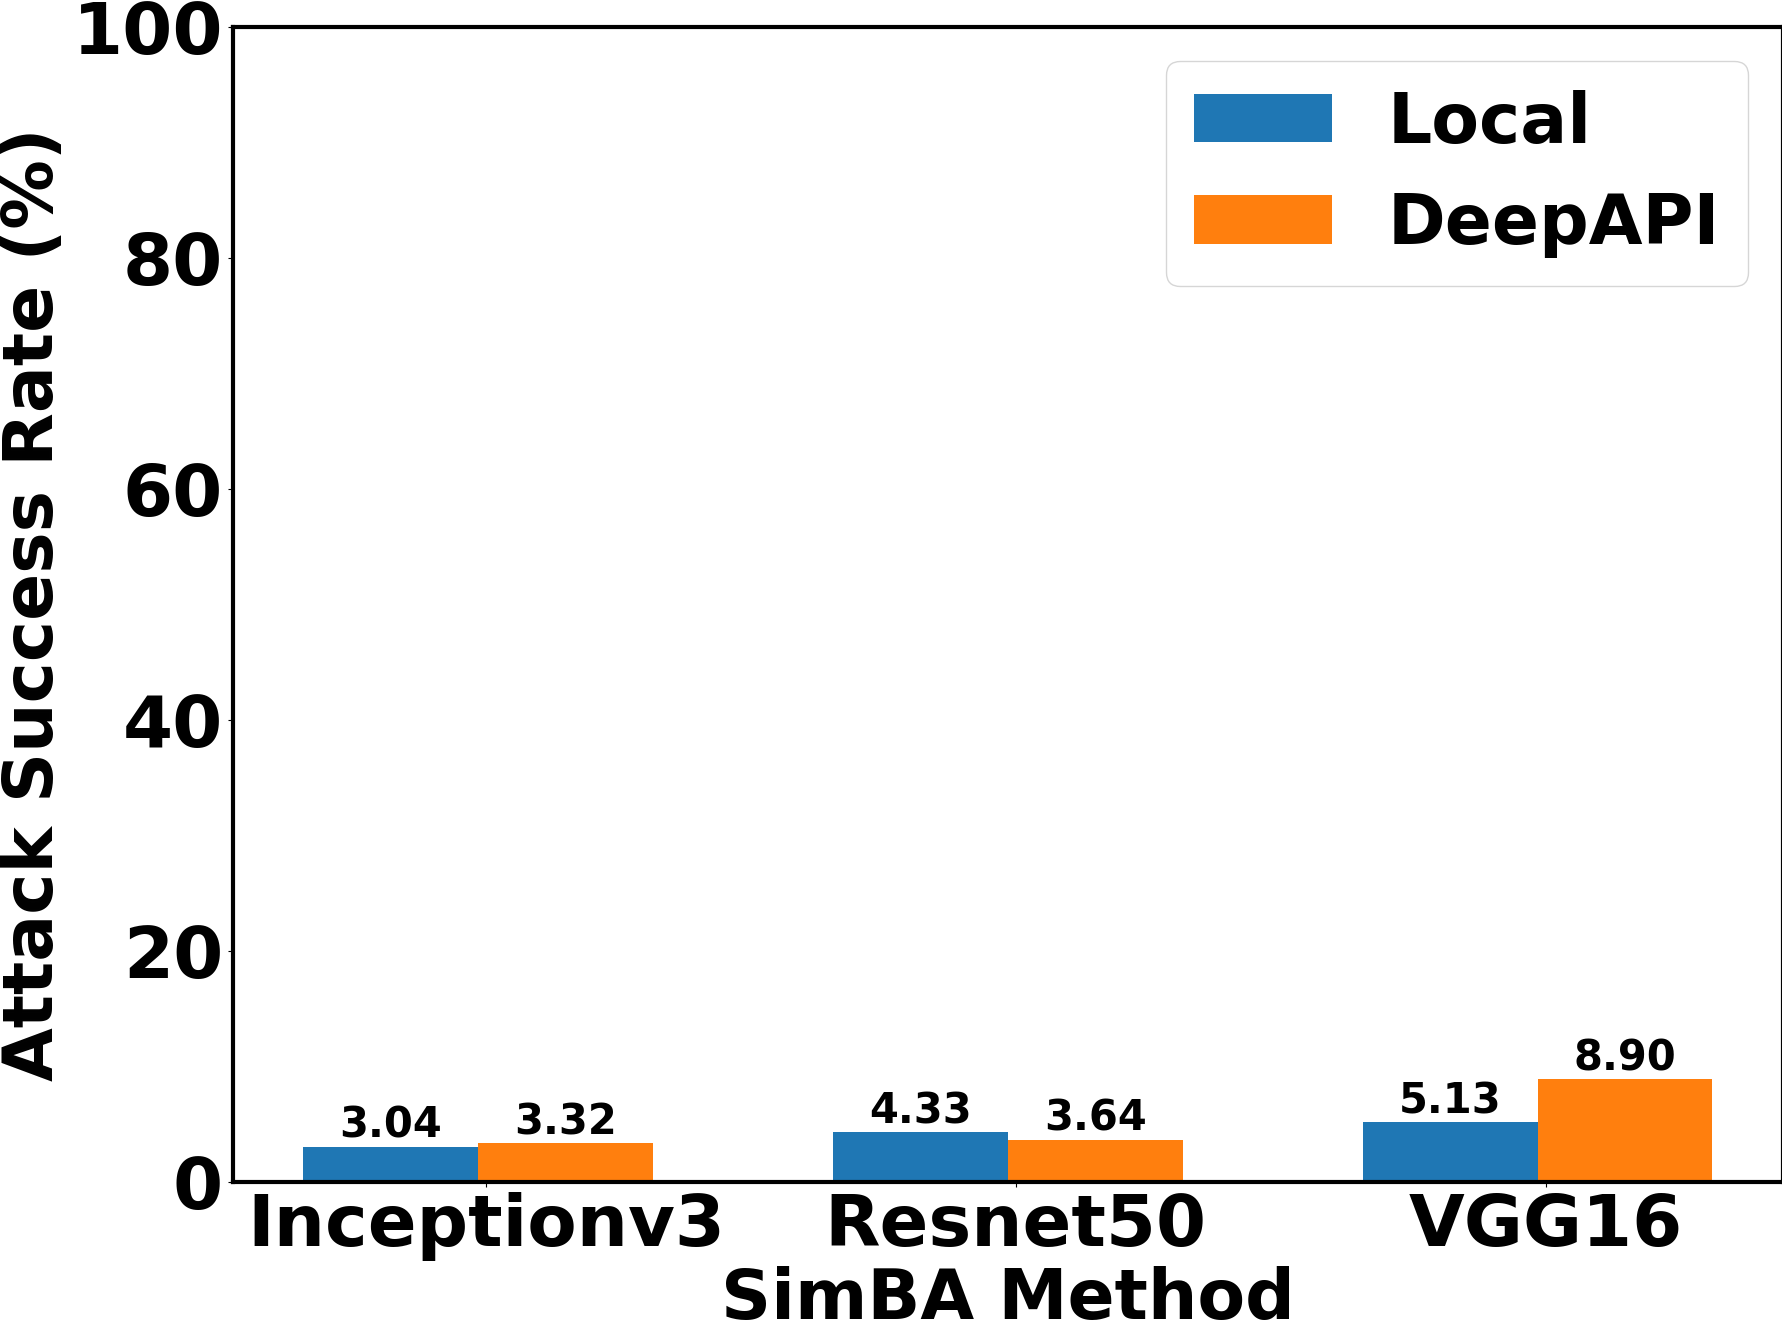
\includegraphics[width=\textwidth]{figures/chapter_classification/simba_attack_success_rate.png}
    \caption{SimBA (Baseline)}
    \label{fig:simba_suc}
\end{subfigure}
\hfill
\begin{subfigure}[b]{0.31\textwidth}
    \centering
    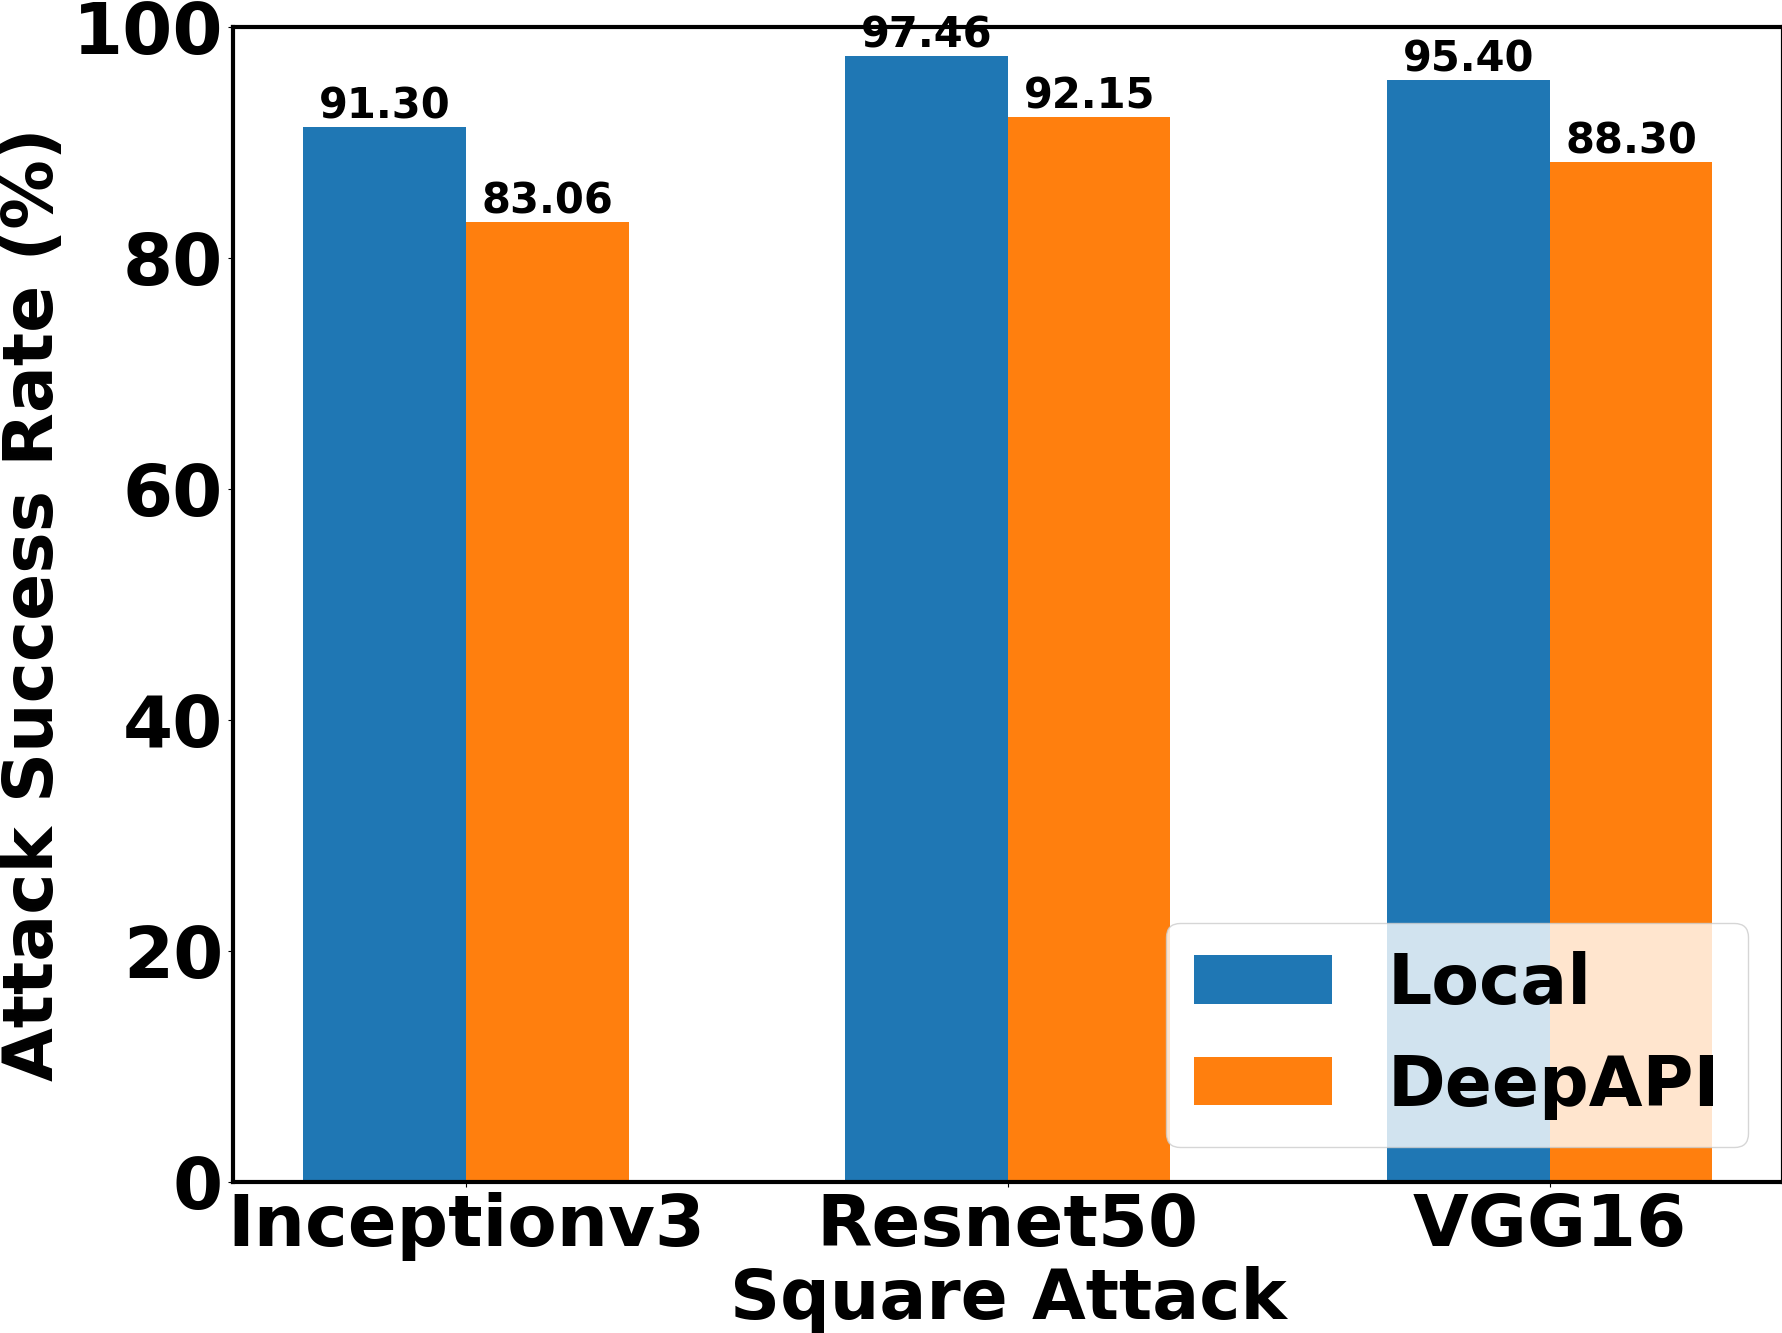
\includegraphics[width=\textwidth]{figures/chapter_classification/square_attack_success_rate.png}
    \caption{Square Attack}
    \label{fig:square_suc}
\end{subfigure}
\hfill
\begin{subfigure}[b]{0.31\textwidth}
    \centering
    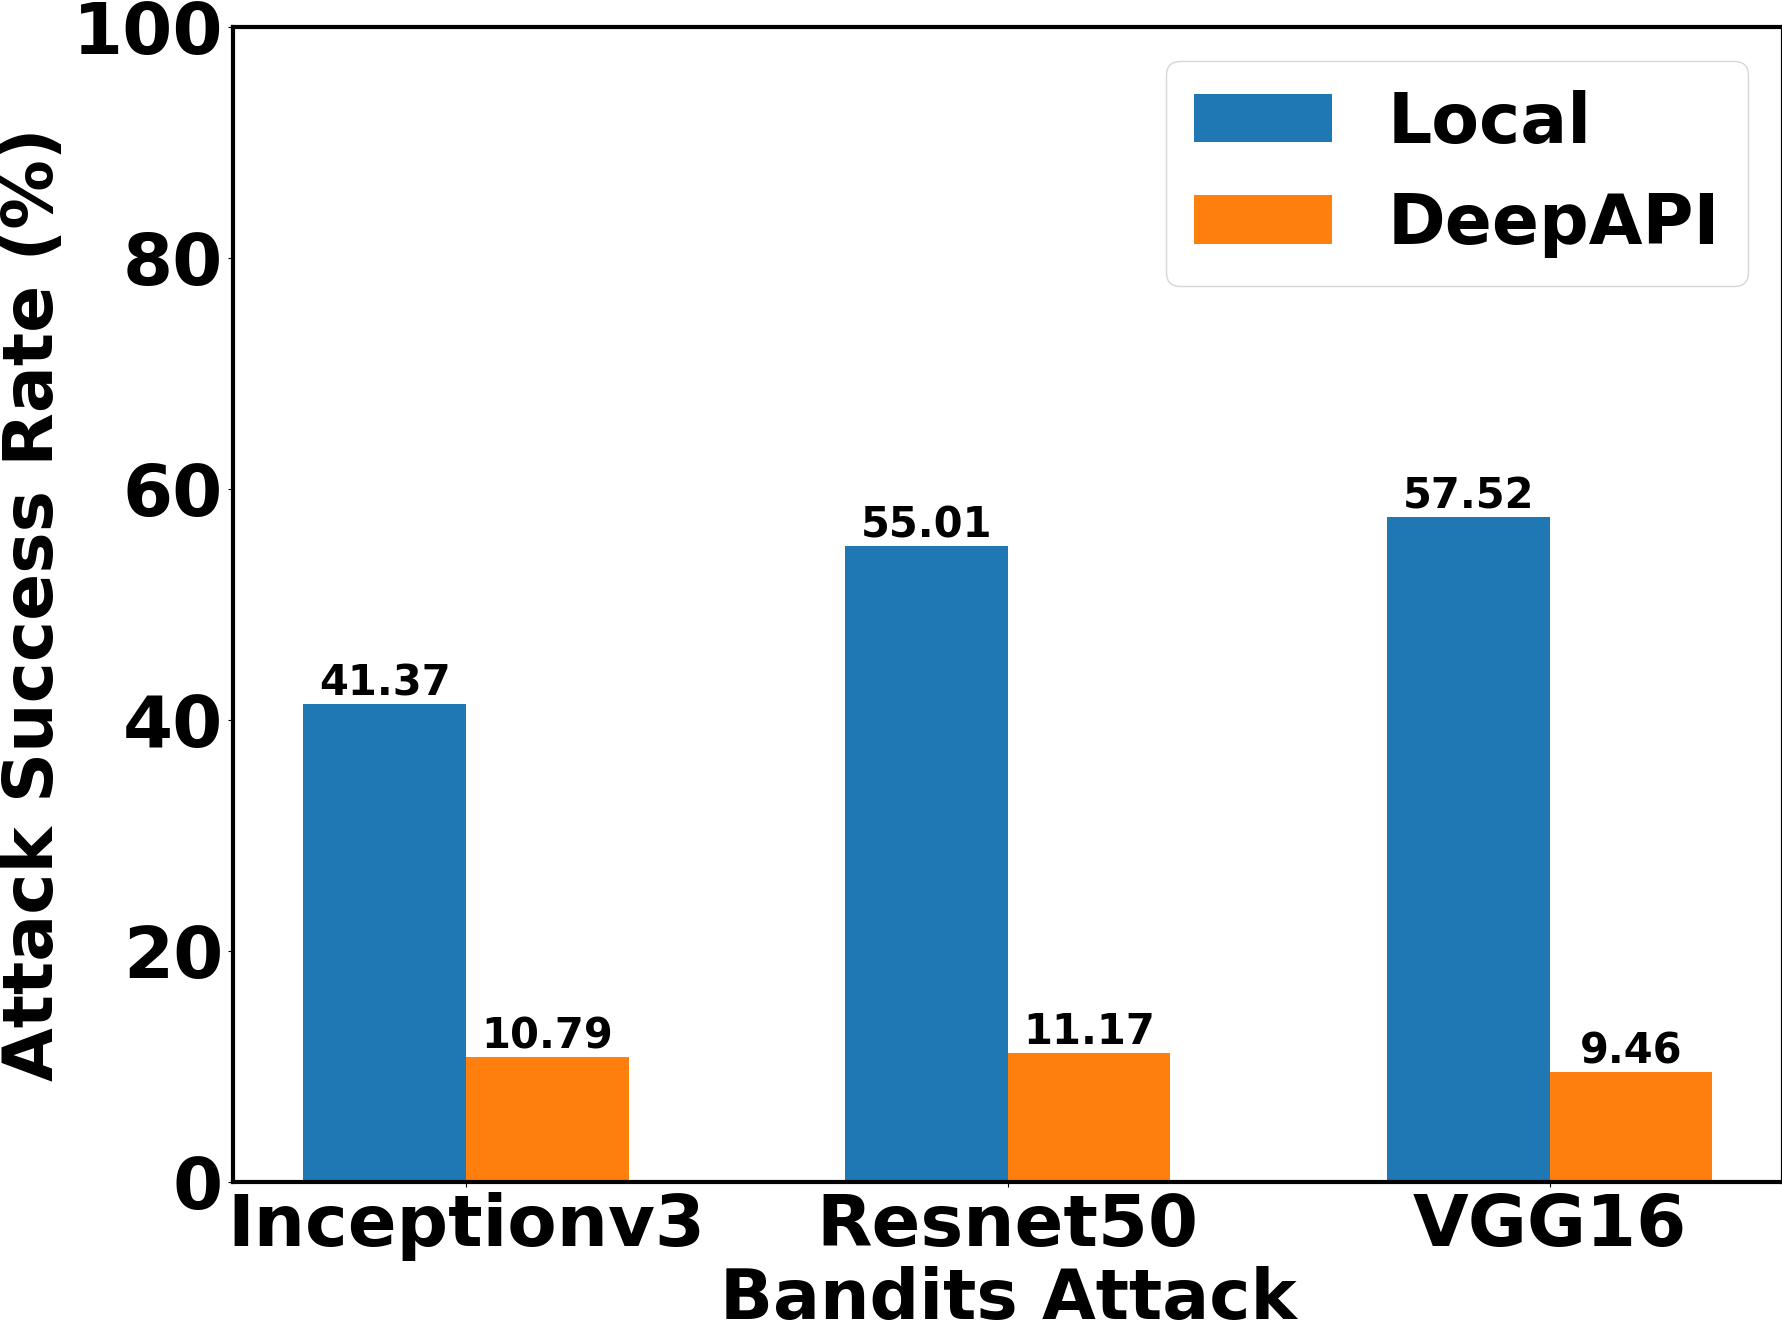
\includegraphics[width=\textwidth]{figures/chapter_classification/bandits_attack_success_rate.png}
    \caption{Bandits Attack}
    \label{fig:bandits_suc}
\end{subfigure}
\caption{The attack success rate tested on local models and cloud APIs.}
\label{fig.suc}
\end{figure*}

\begin{figure*}[bth]
\centering
\begin{subfigure}[b]{0.31\textwidth}
    \centering
    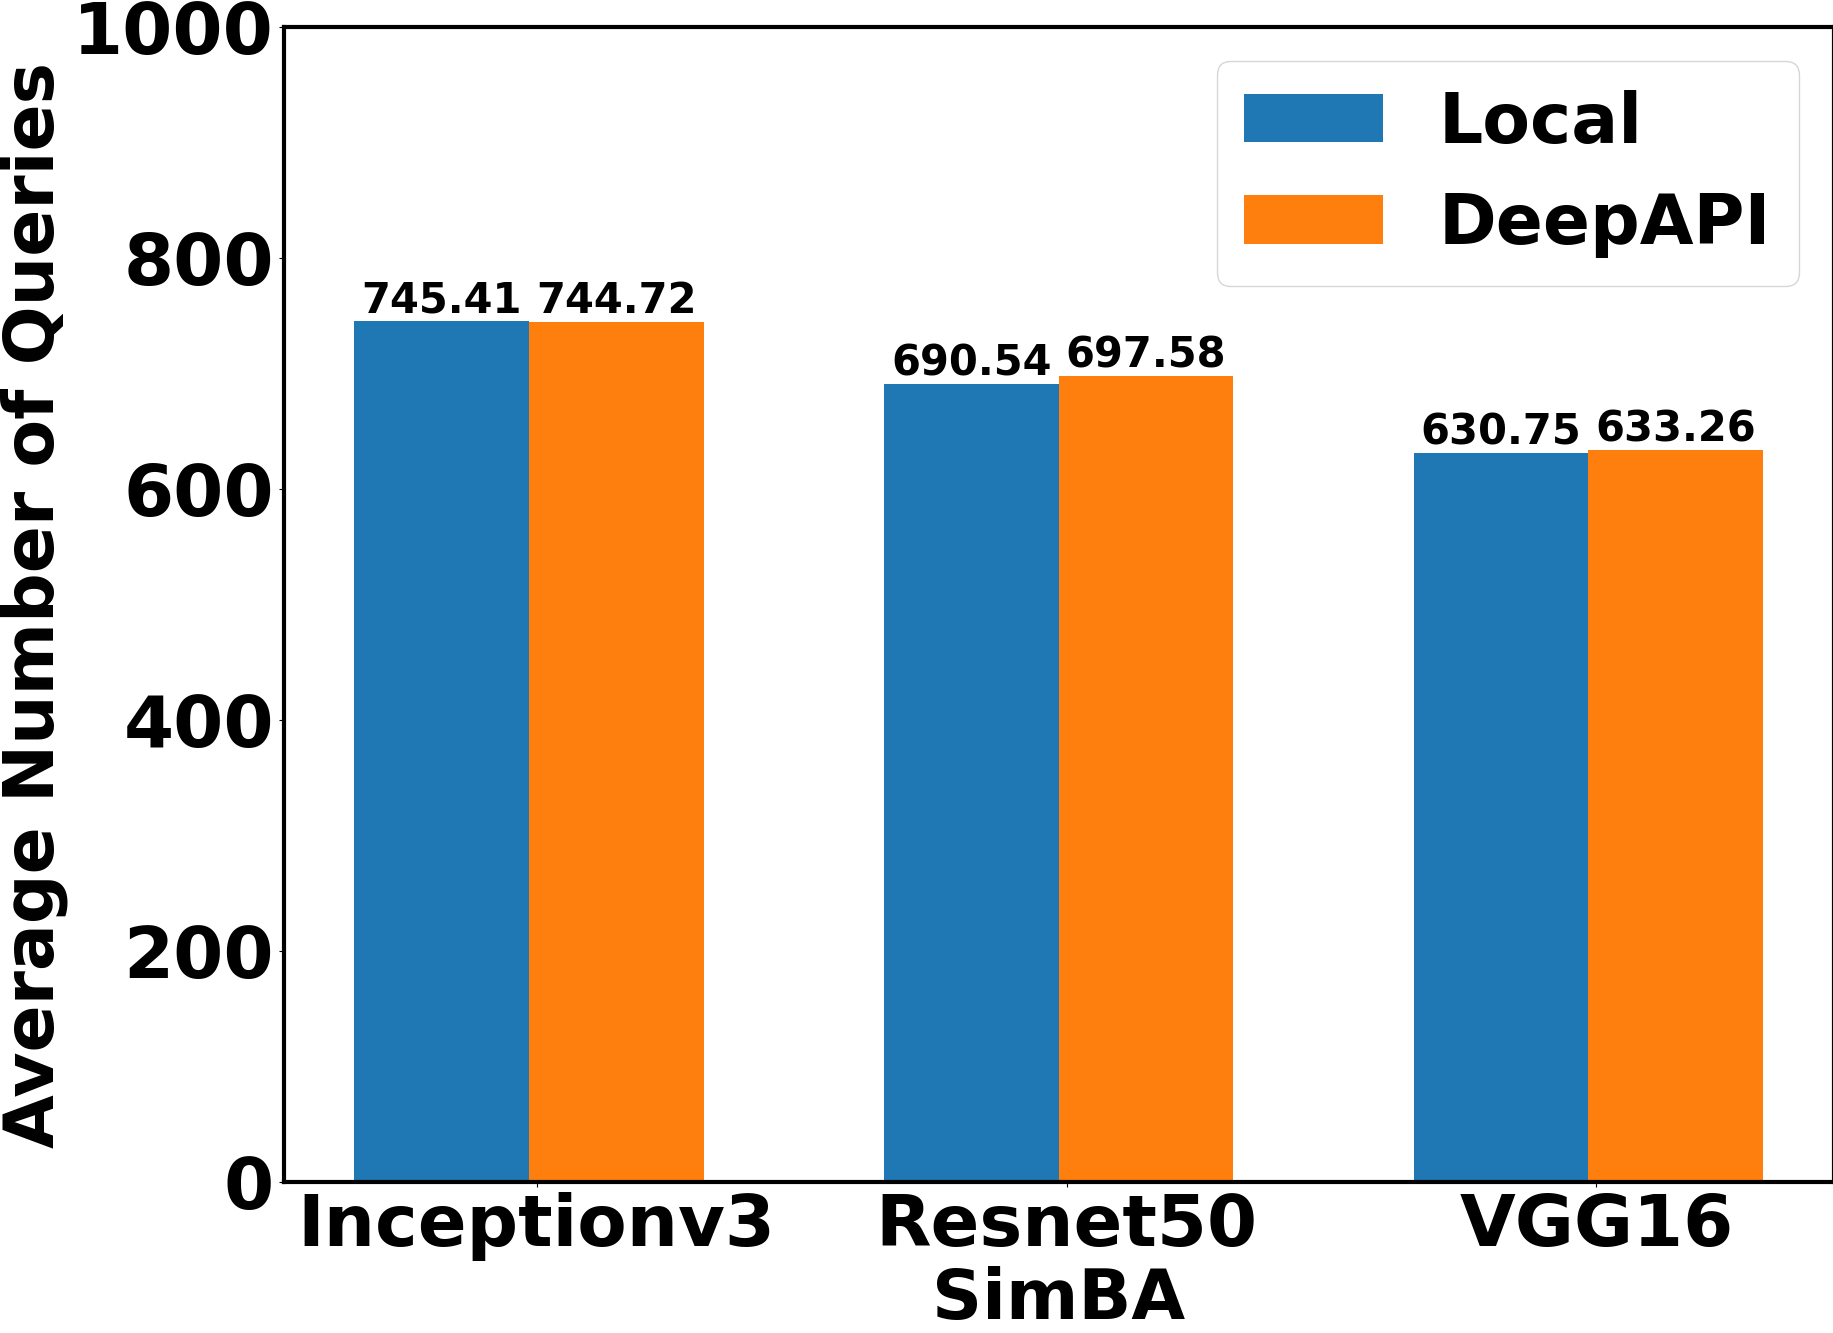
\includegraphics[width=\textwidth]{figures/chapter_classification/simba_number_of_queries.png}
    \caption{SimBA (Baseline)}
    \label{fig:simba_queries}
\end{subfigure}
\hfill
\begin{subfigure}[b]{0.31\textwidth}
    \centering
    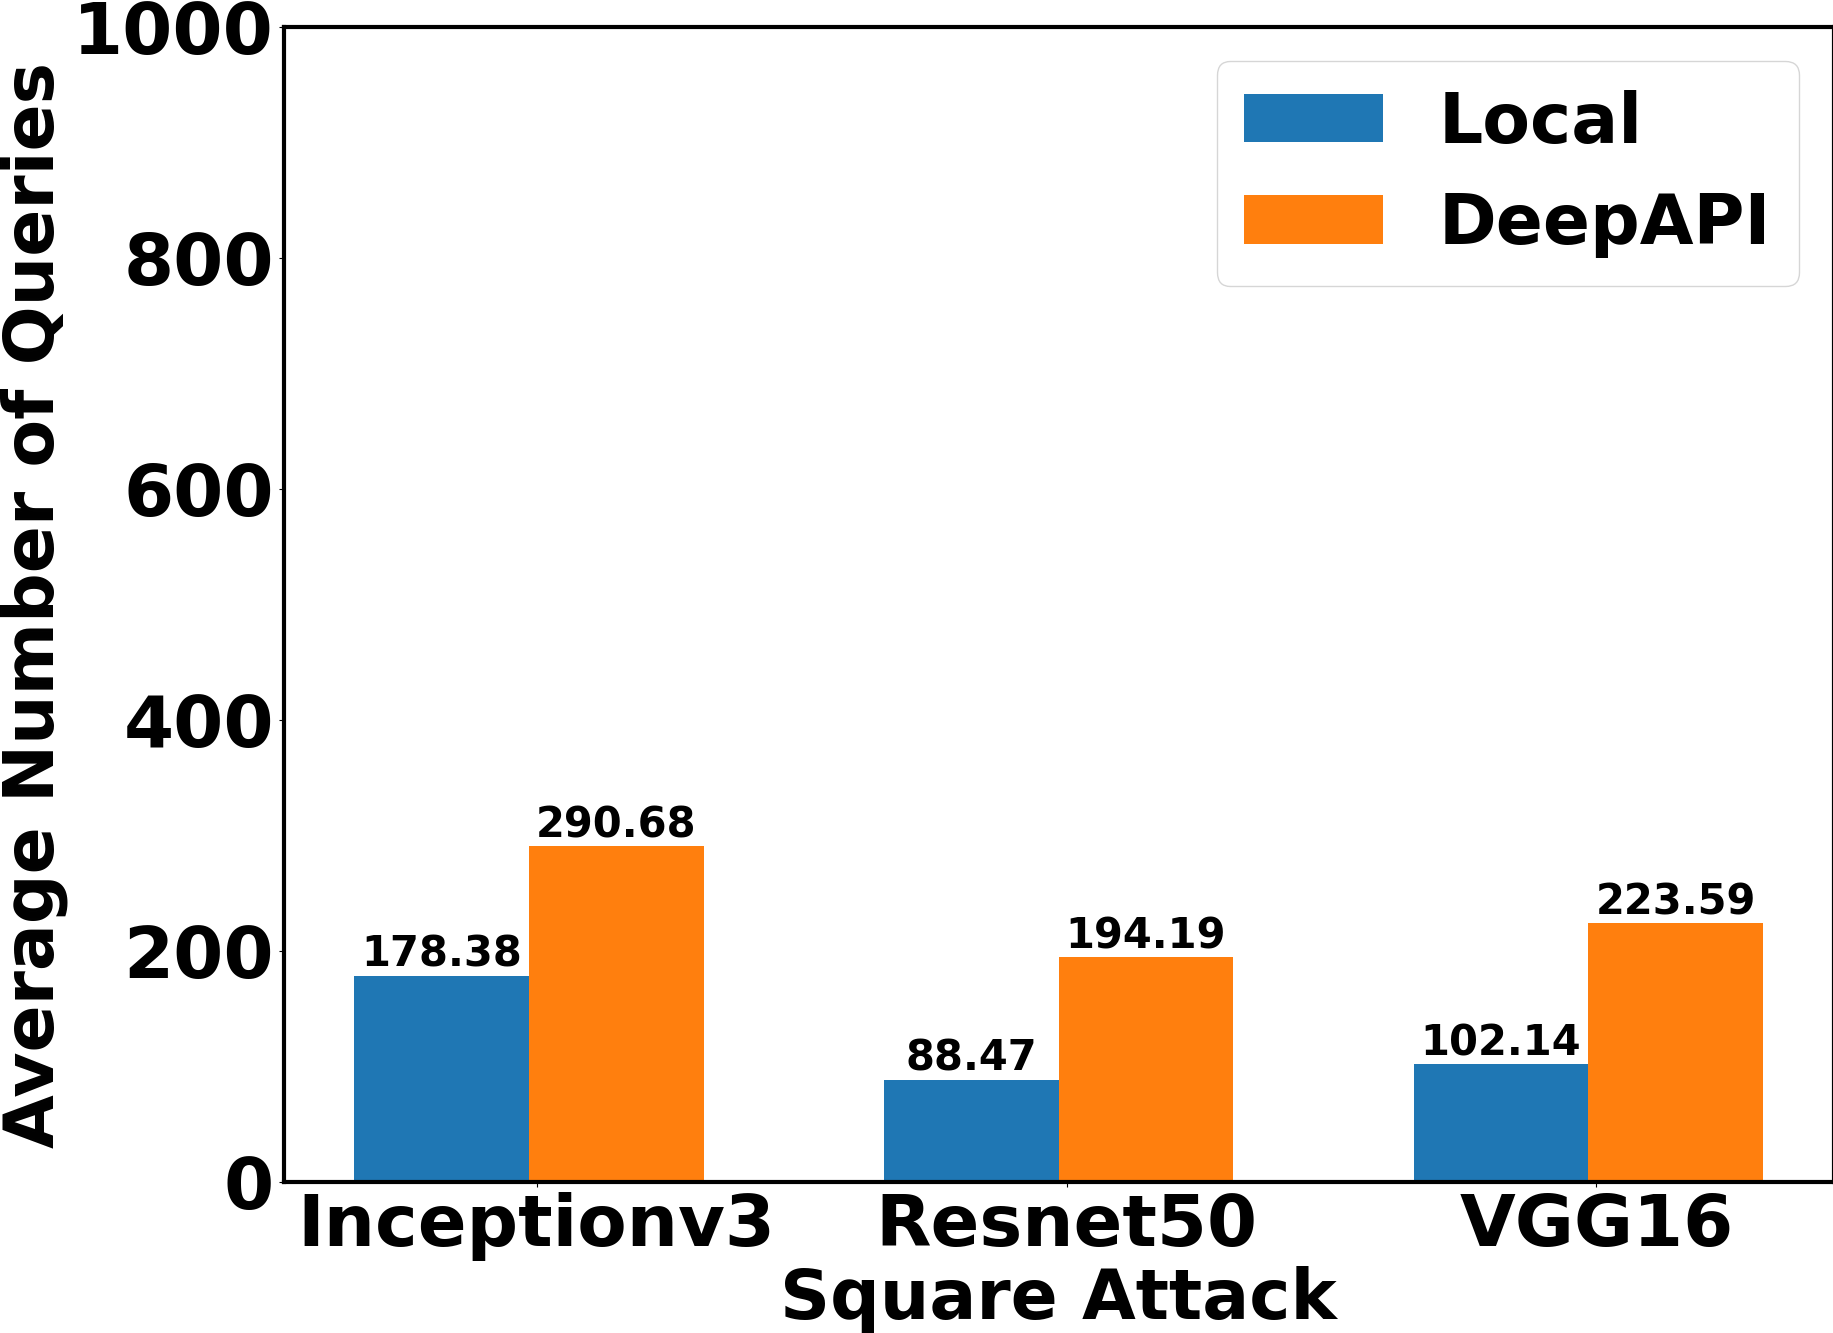
\includegraphics[width=\textwidth]{figures/chapter_classification/square_number_of_queries.png}
    \caption{Square Attack}
    \label{fig:square_queries}
\end{subfigure}
\hfill
\begin{subfigure}[b]{0.31\textwidth}
    \centering
    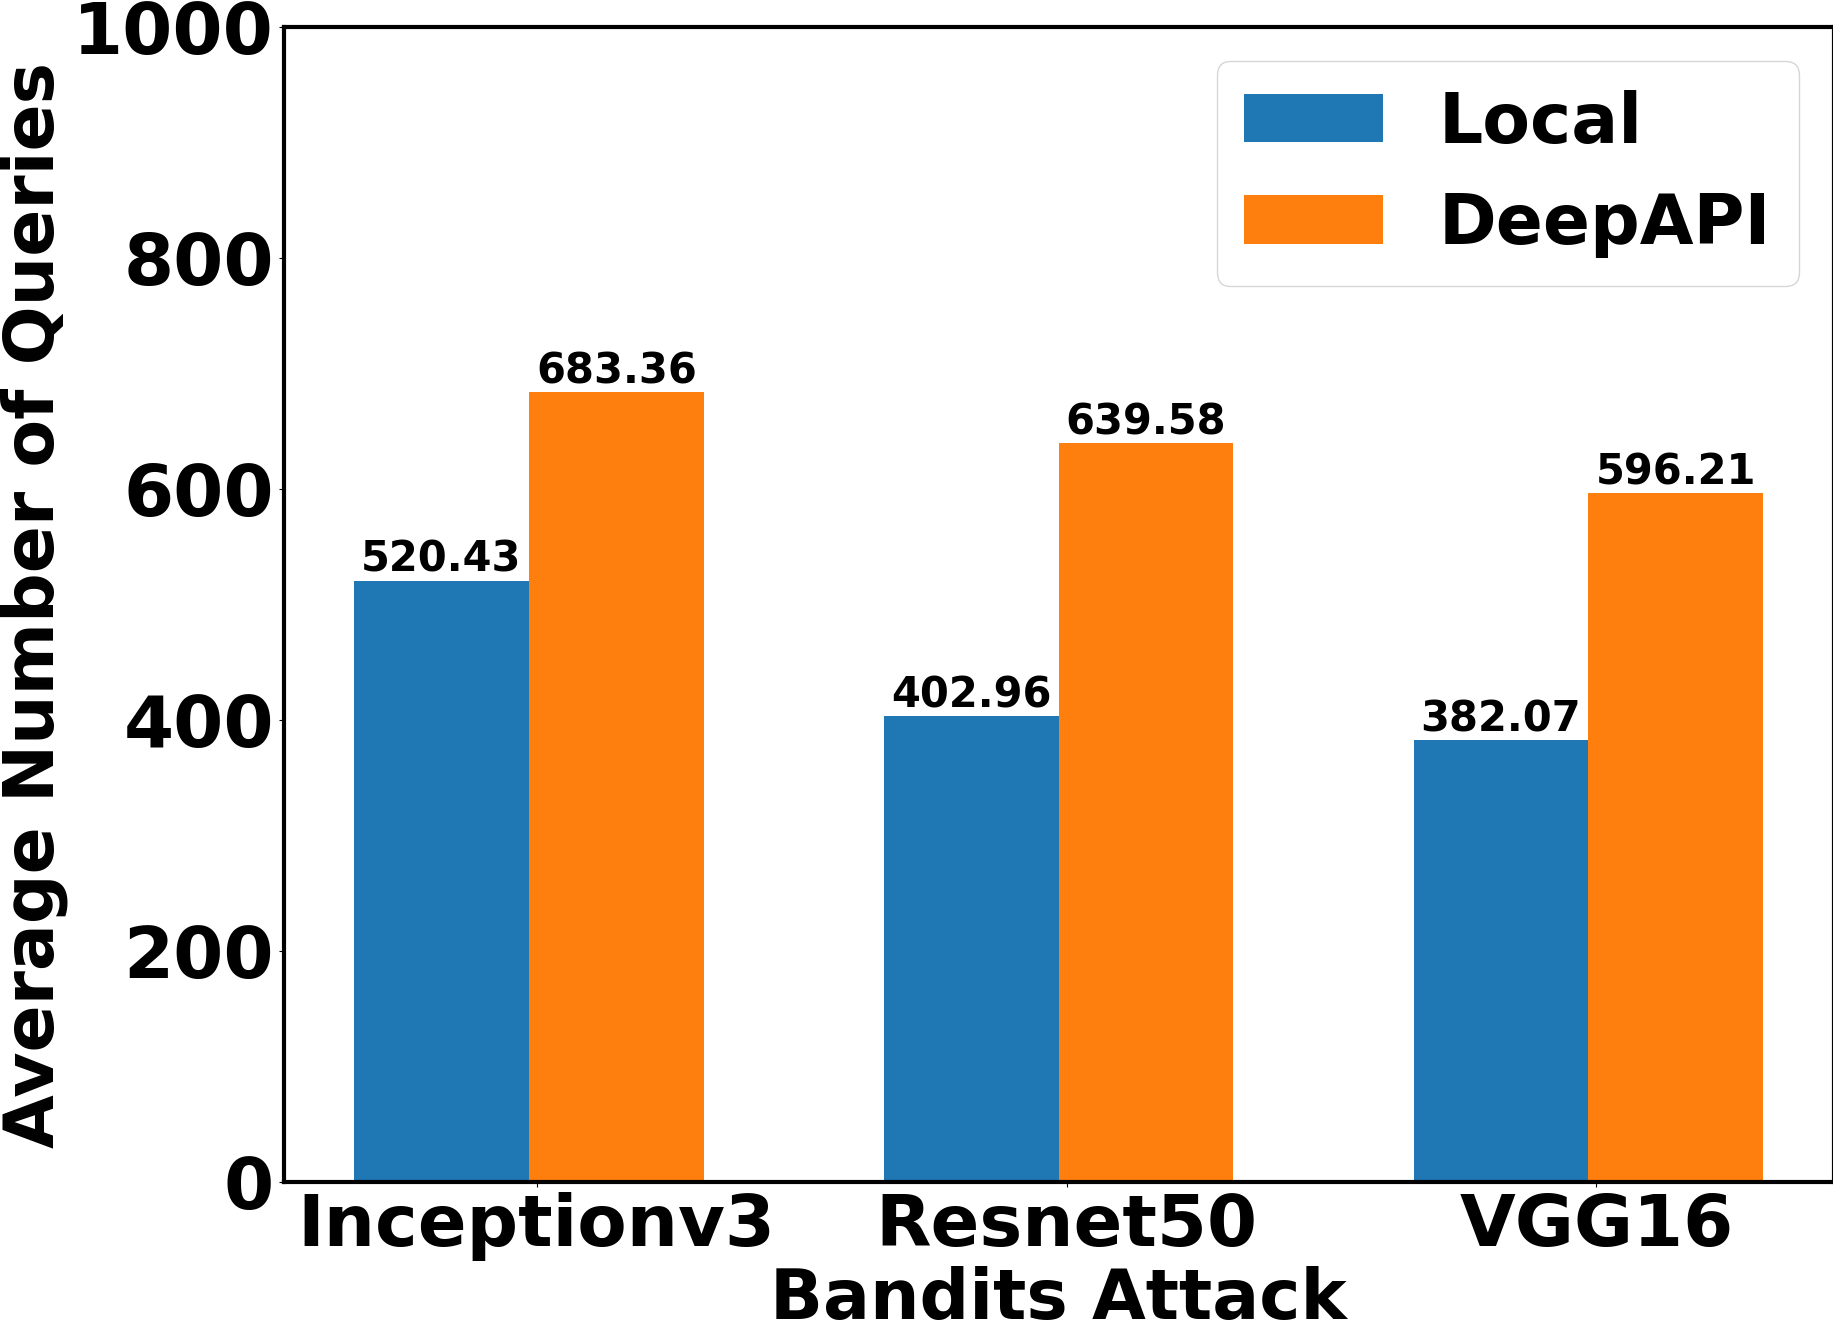
\includegraphics[width=\textwidth]{figures/chapter_classification/bandits_number_of_queries.png}
    \caption{Bandits Attack}
    \label{fig:bandits_queries}
\end{subfigure}
\caption{The average number of queries tested on local models and cloud APIs}
\label{fig.queries}
\end{figure*}

% \clearpage

\subsection{Horizontal Distribution}

In this section, we measure the effect of horizontal distribution on the number of queries and the attack success rate. We sampled 100 images from the ImageNet dataset \citep{moore2020fiftyone} and tested three online black-box attacks against three image classification models \citep{chollet2015keras}.

As shown in Tables \ref{tab:non} and \ref{tab:horizon}, while there is a slight variation in the average number of queries after applying horizontal distribution, this is mainly due to discrepancies in the pseudo-random number generator. This variation is insignificant because horizontal distribution does not change how the attack method generates adversarial perturbations.

% \begin{table}[bh]
% \begin{center}
% \begin{tabular}{cccccccccc}
% \hline
% Attacks & \multicolumn{6}{c}{Average Number of Queries} \\ \hline
%         & \multicolumn{2}{c}{Inceptionv3}           & \multicolumn{2}{c}{ResNet50}             & \multicolumn{2}{c}{VGG16}         \\
%         \hline
%         & Without & With  & Without & With  & Without & With \\
%         \hline
% SimBA (Baseline Method)   & 775 &  & 740  &  & 730 \\
% Square (Local Search)  & 360 &  & 200  &  & 228  \\
% Bandits (Gradient Estimation) & 732 &  & 688 &  & 698 \\ \hline
% \end{tabular}
% \end{center}
% \caption{The average number of queries with and without horizontal distribution.}
% \label{tab:non}
% \end{table}

We further evaluate the impact of horizontal distribution on the total attack time. As shown in Fig. \ref{fig.horizon_time}, horizontal distribution significantly reduces the total attack time for all the attacks. By sending concurrent queries across multiple images, we can achieve a successful attack faster without increasing the query budget. The acceleration ratio depends on the number of computational nodes deployed for the cloud API. Deploying more nodes behind the load balancer can lead to a larger acceleration ratio.

\begin{table}[bth]
\begin{center}
\begin{tabular}{cccccccccc}
\hline
Attacks & \multicolumn{3}{c}{Average Number of Queries} \\ \hline
        & Inceptionv3           & ResNet50             & VGG16         \\
SimBA (Baseline Method)   & 775   & 740    & 730  \\
Square (Local Search)  & 360   & 200    & 228  \\
Bandits (Gradient Estimation) & 732   & 688   & 698 \\ \hline
\end{tabular}
\end{center}
\caption{The average number of queries of non-distributed attacks.}
\label{tab:non}
\end{table}

\begin{table}[bth]
\begin{center}
\begin{tabular}{cccccccccc}
\hline
Attacks & \multicolumn{3}{c}{Average Number of Queries}\\ \hline
        & Inceptionv3           & ResNet50             & VGG16         \\
SimBA (Baseline Method)   &  773  & 779    & 728  \\
Square (Local Search)  & 360   & 205    & 223  \\
Bandits (Gradient Estimation) & 740   & 673  & 707  \\ \hline
\end{tabular}
\end{center}
\caption{The average number of queries of horizontally distributed attacks.}
\label{tab:horizon}
\end{table}

In summary, our experiments showed that horizontal distribution reduced the total attack time by a factor of five on average and have little affect the attack success rate and the number of queries. This suggests that horizontal distribution can bring black-box attacks closer to being a practical threat, by achieving faster attacks without increasing the query budget.

% In summary, our experiments showed that horizontal distribution reduced the total attack time by a factor of five on average and did not significantly affect the attack success rate and the average number of queries, which brings black-box attacks a step closer to be a practical threat.

\begin{figure*}[tbhp]
\centering
\begin{subfigure}[b]{0.32\textwidth}
    \centering
    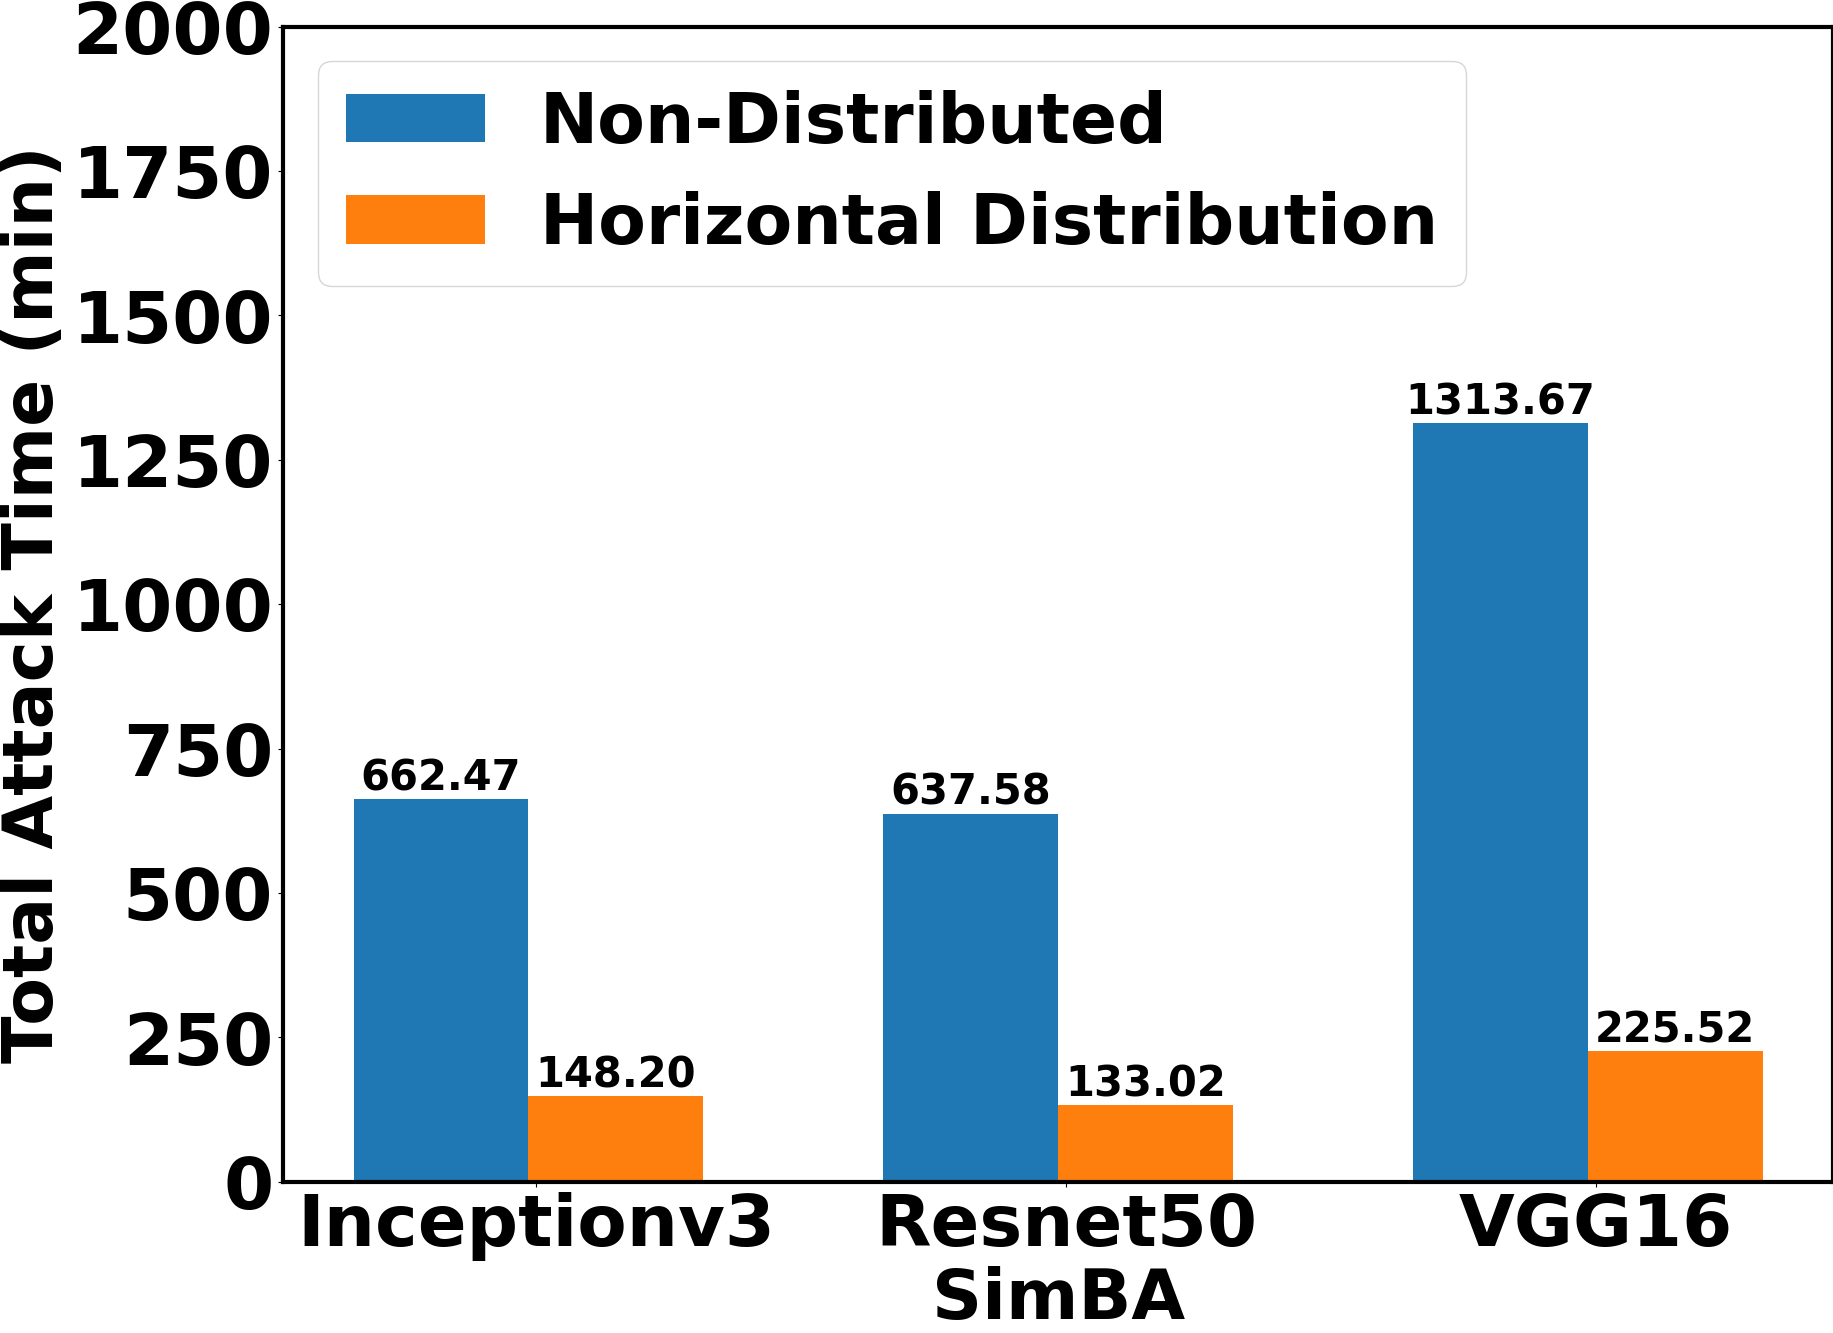
\includegraphics[width=\textwidth]{figures/chapter_classification/simba_attack_horizontal_time.png}
    \caption{SimBA (Baseline)}
    \label{fig:simba_horizon}
\end{subfigure}
\hfill
\begin{subfigure}[b]{0.32\textwidth}
    \centering
    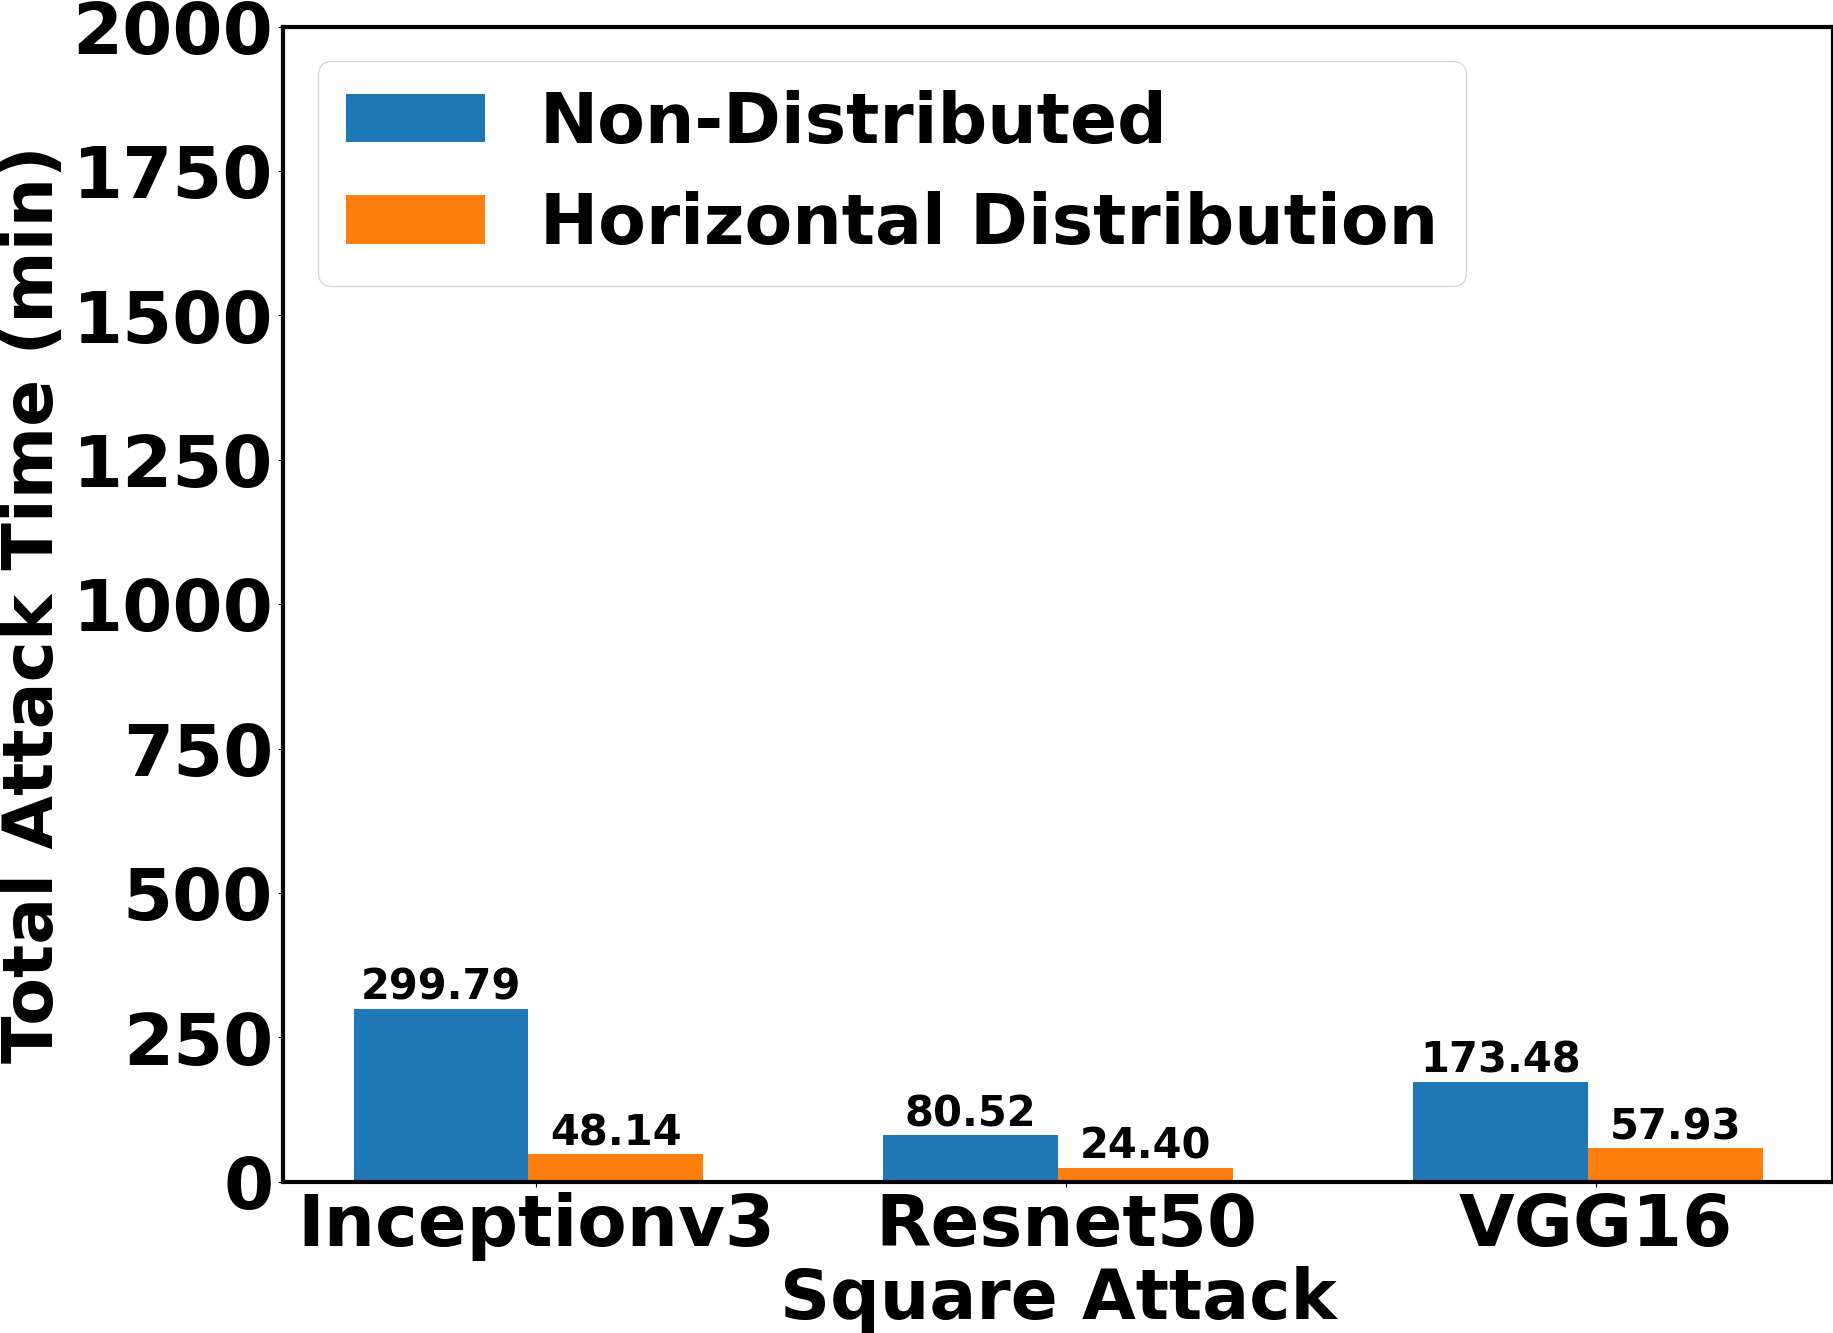
\includegraphics[width=\textwidth]{figures/chapter_classification/square_attack_horizontal_time.png}
    \caption{Square Attack}
    \label{fig:square_horizon}
\end{subfigure}
\hfill
\begin{subfigure}[b]{0.32\textwidth}
    \centering
    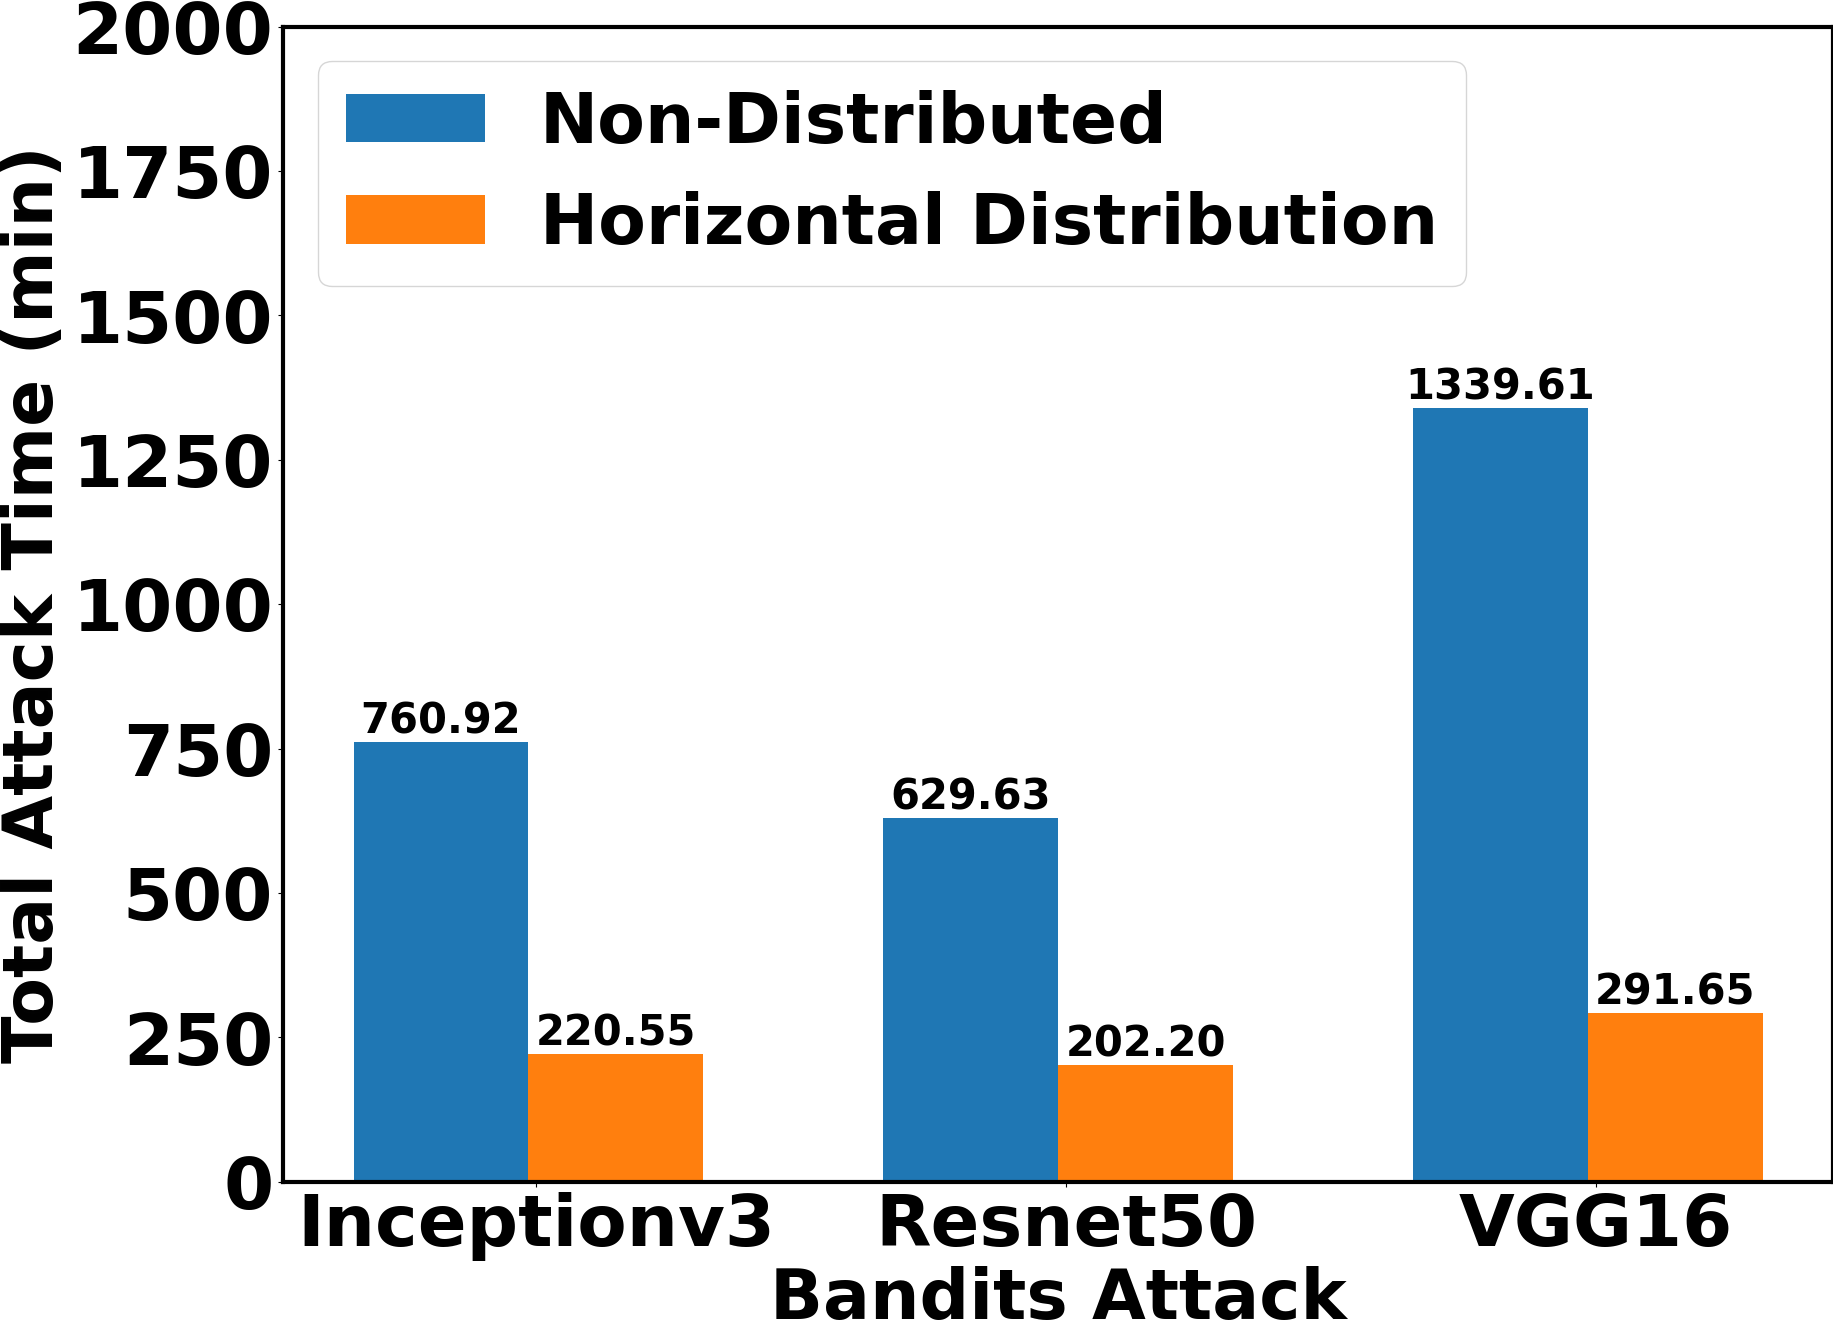
\includegraphics[width=\textwidth]{figures/chapter_classification/bandits_attack_horizontal_time.png}
    \caption{Bandits Attack}
    \label{fig:bandits_horizon}
\end{subfigure}
\caption{The total attack time with and without horizontal distribution.}
\label{fig.horizon_time}
\end{figure*}

% \clearpage

\subsection{Vertical Distribution}

In this section, we focus on improving the efficiency of attacking a single image through vertical distribution. The vertical distribution sends out queries concurrently across iterations of the same image. The implementations of vertical distribution presented in Section \ref{horizon_vertical} serve to illustrate the general concept of distributed attacks, but there may be other approaches to achieving vertical distribution that are more effective for specific black-box attacks. In the following experiments, we use the implementation presented in Section \ref{horizon_vertical}.

% In this section, we focus on improving the iteration process for attacking a single image using vertical distribution. The vertical distribution accelerates the attack by concurrently sending out queries across iterations of the same image. In the following experiments, We use examples of vertical distribution illustrated in Section \ref{horizon_vertical}, while there are different ways to achieve vertical distribution for a specific black-box attack.

\textbf{The SimBA Attack}: Using vertical distribution, we can reduce the probability of the highest ground-truth class more quickly within a limited time by randomly choosing a batch of unrepeated pixels to perturb (see Fig. \ref{fig:simba_plot}).  This is particularly effective when attacking with SimBA, which has a relatively low attack success rate. 

% Though the baseline method, SimBA, achieves a relatively low attack success rate, we can use vertical distribution to decrease the probability of the correct class faster until the model makes a wrong prediction. 

\textbf{The Square Attack}: Similarly, the vertically distributed square attack decreases the margin loss faster than the original method and achieves an early successful attack (see Fig. \ref{fig:square_plot}). This is because multiple square-shaped perturbations are generated as a batch in a single iteration, which accelerates and increases the attack success rate. 

\textbf{The Bandits Attack}: The vertically distributed bandits attack also achieves an early successful attack (see Fig. \ref{fig:bandits_plot}). Note that the original non-distributed bandits attack failed to generate an adversarial example after 1,000 queries, which means vertically distributed attacks can also improve the attack success rate.

% \clearpage

% \begin{figure*}[t]
% \centering
% \begin{subfigure}[t]{0.3\textwidth}
%     \centering
%     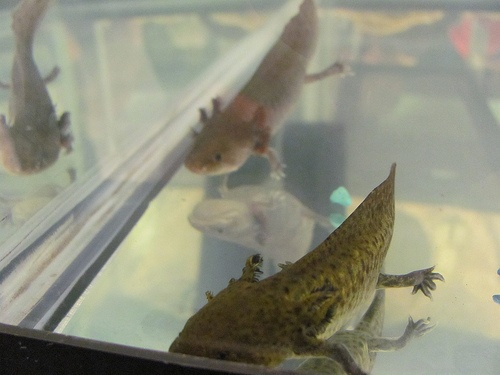
\includegraphics[width=\textwidth]{figures/chapter_classification/x_29_adv_simba_1.jpg}
%     \caption{SimBA (No Distribution)}
%     \label{fig:simba_no_img}
% \end{subfigure}
% \hfill
% \begin{subfigure}[t]{0.3\textwidth}
%     \centering
%     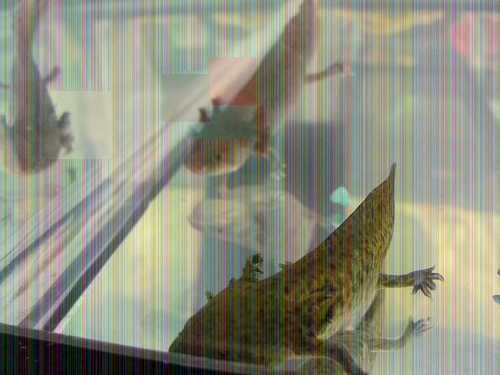
\includegraphics[width=\textwidth]{figures/chapter_classification/x_29_adv_square_1.jpg}
%     \caption{Square Attack (No Distribution)}
%     \label{fig:square_no_img}
% \end{subfigure}
% \hfill
% \begin{subfigure}[t]{0.3\textwidth}
%     \centering
%     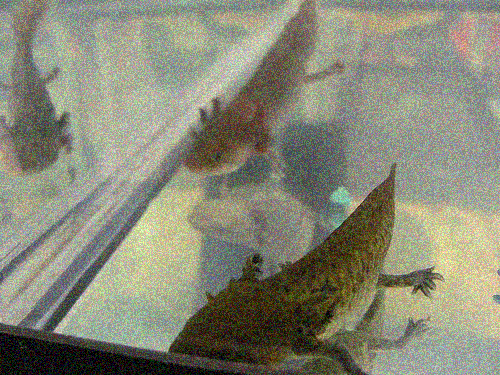
\includegraphics[width=\textwidth]{figures/chapter_classification/x_29_adv_bandits_1.jpg}
%     \caption{Bandits Attack (No Distribution)}
%     \label{fig:bandits_no_img}
% \end{subfigure}
% \hfill
% \begin{subfigure}[t]{0.3\textwidth}
%     \centering
%     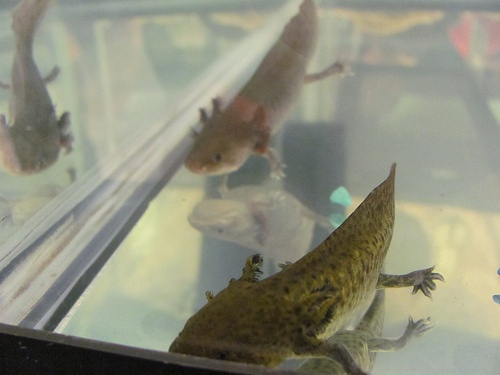
\includegraphics[width=\textwidth]{figures/chapter_classification/x_29_adv_simba_8.jpg}
%     \caption{SimBA (Vertical)}
%     \label{fig:simba_vertical_img}
% \end{subfigure}
% \hfill
% \begin{subfigure}[t]{0.3\textwidth}
%     \centering
%     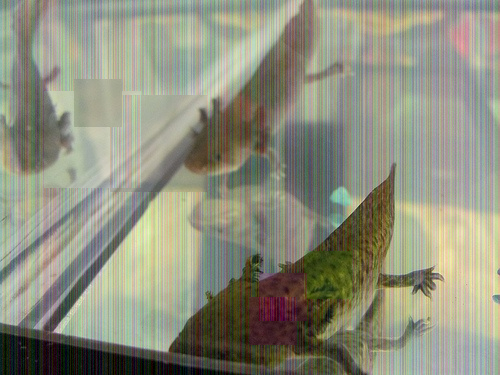
\includegraphics[width=\textwidth]{figures/chapter_classification/x_29_adv_square_8.jpg}
%     \caption{Square Attack (Vertical)}
%     \label{fig:square_vertical_img}
% \end{subfigure}
% \hfill
% \begin{subfigure}[t]{0.3\textwidth}
%     \centering
%     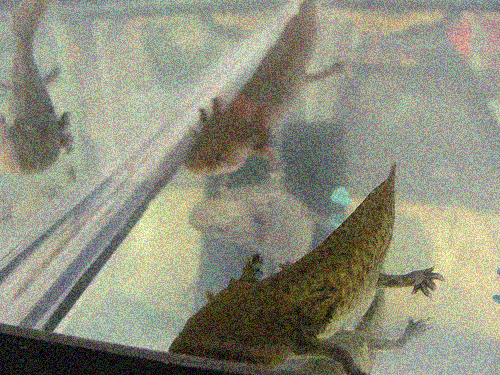
\includegraphics[width=\textwidth]{figures/chapter_classification/x_29_adv_bandits_8.jpg}
%     \caption{Bandits Attack (Vertical)}
%     \label{fig:bandits_vertical_img}
% \end{subfigure}
% \caption{Adversarial examples generated by different black-box attacks.}
% \label{fig.vertical_img}
% \end{figure*}

% Besides, we show some adversarial images generated by vertically distributed black-box attacks and original methods in Fig. \ref{fig.vertical_img}. They were generated under the same $\epsilon=0.05$, and we cannot tell the difference from the perspective of human eyes.

In conclusion, compared with non-distributed attacks, vertically distributed attacks require less time to achieve a successful attack for each image, while the generated adversarial example is visually the same as in the original method. This highlights the potential of vertical distribution as an effective strategy for improving the efficiency of black-box attacks.

\begin{figure*}[bph]
\centering
\begin{subfigure}[b]{0.32\textwidth}
    \centering
    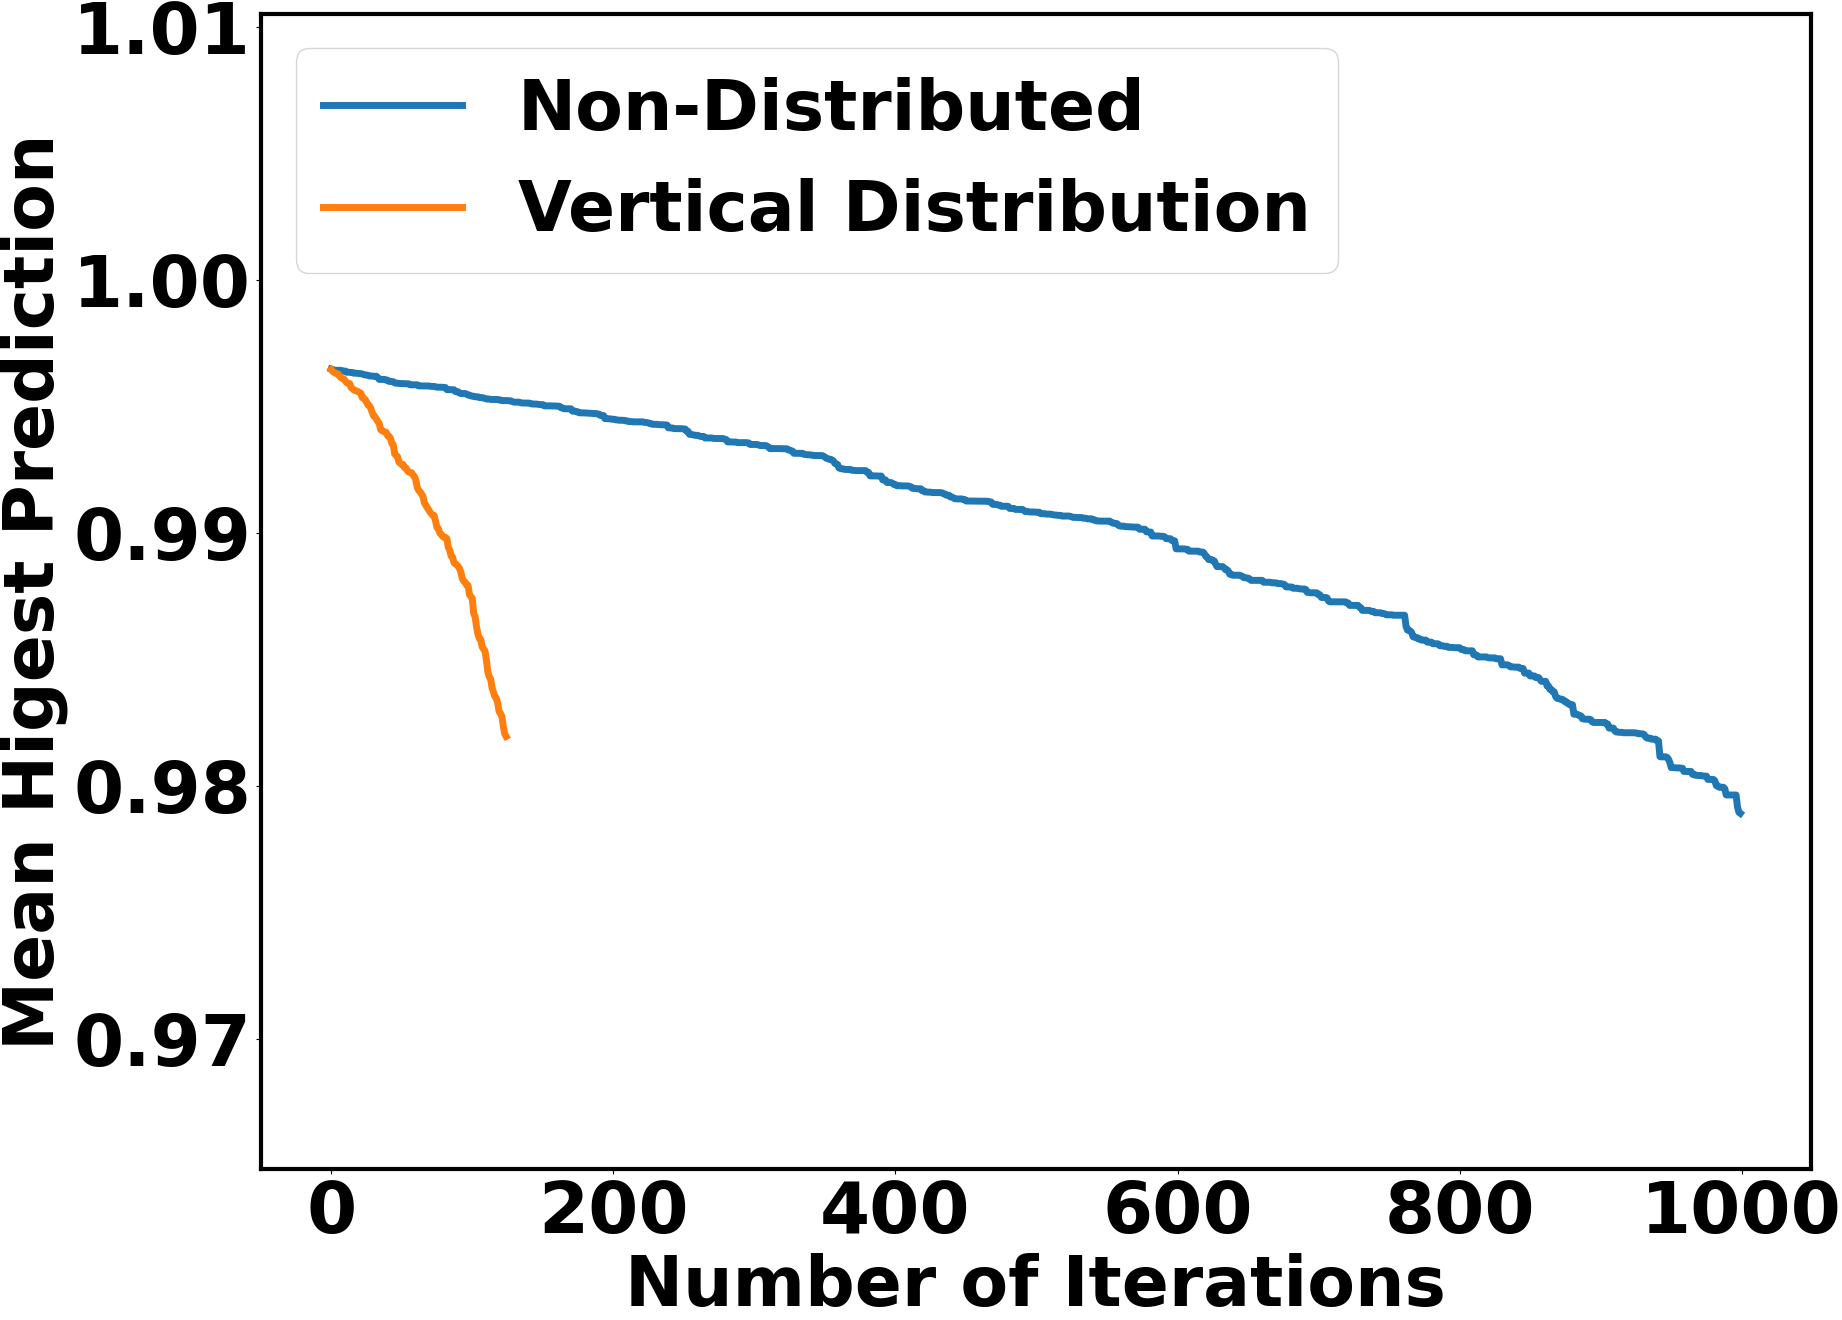
\includegraphics[width=\textwidth]{figures/chapter_classification/simba_attack_vertical_margin.png}
    \caption{SimBA (Baseline)}
    \label{fig:simba_plot}
\end{subfigure}
\hfill
\begin{subfigure}[b]{0.32\textwidth}
    \centering
    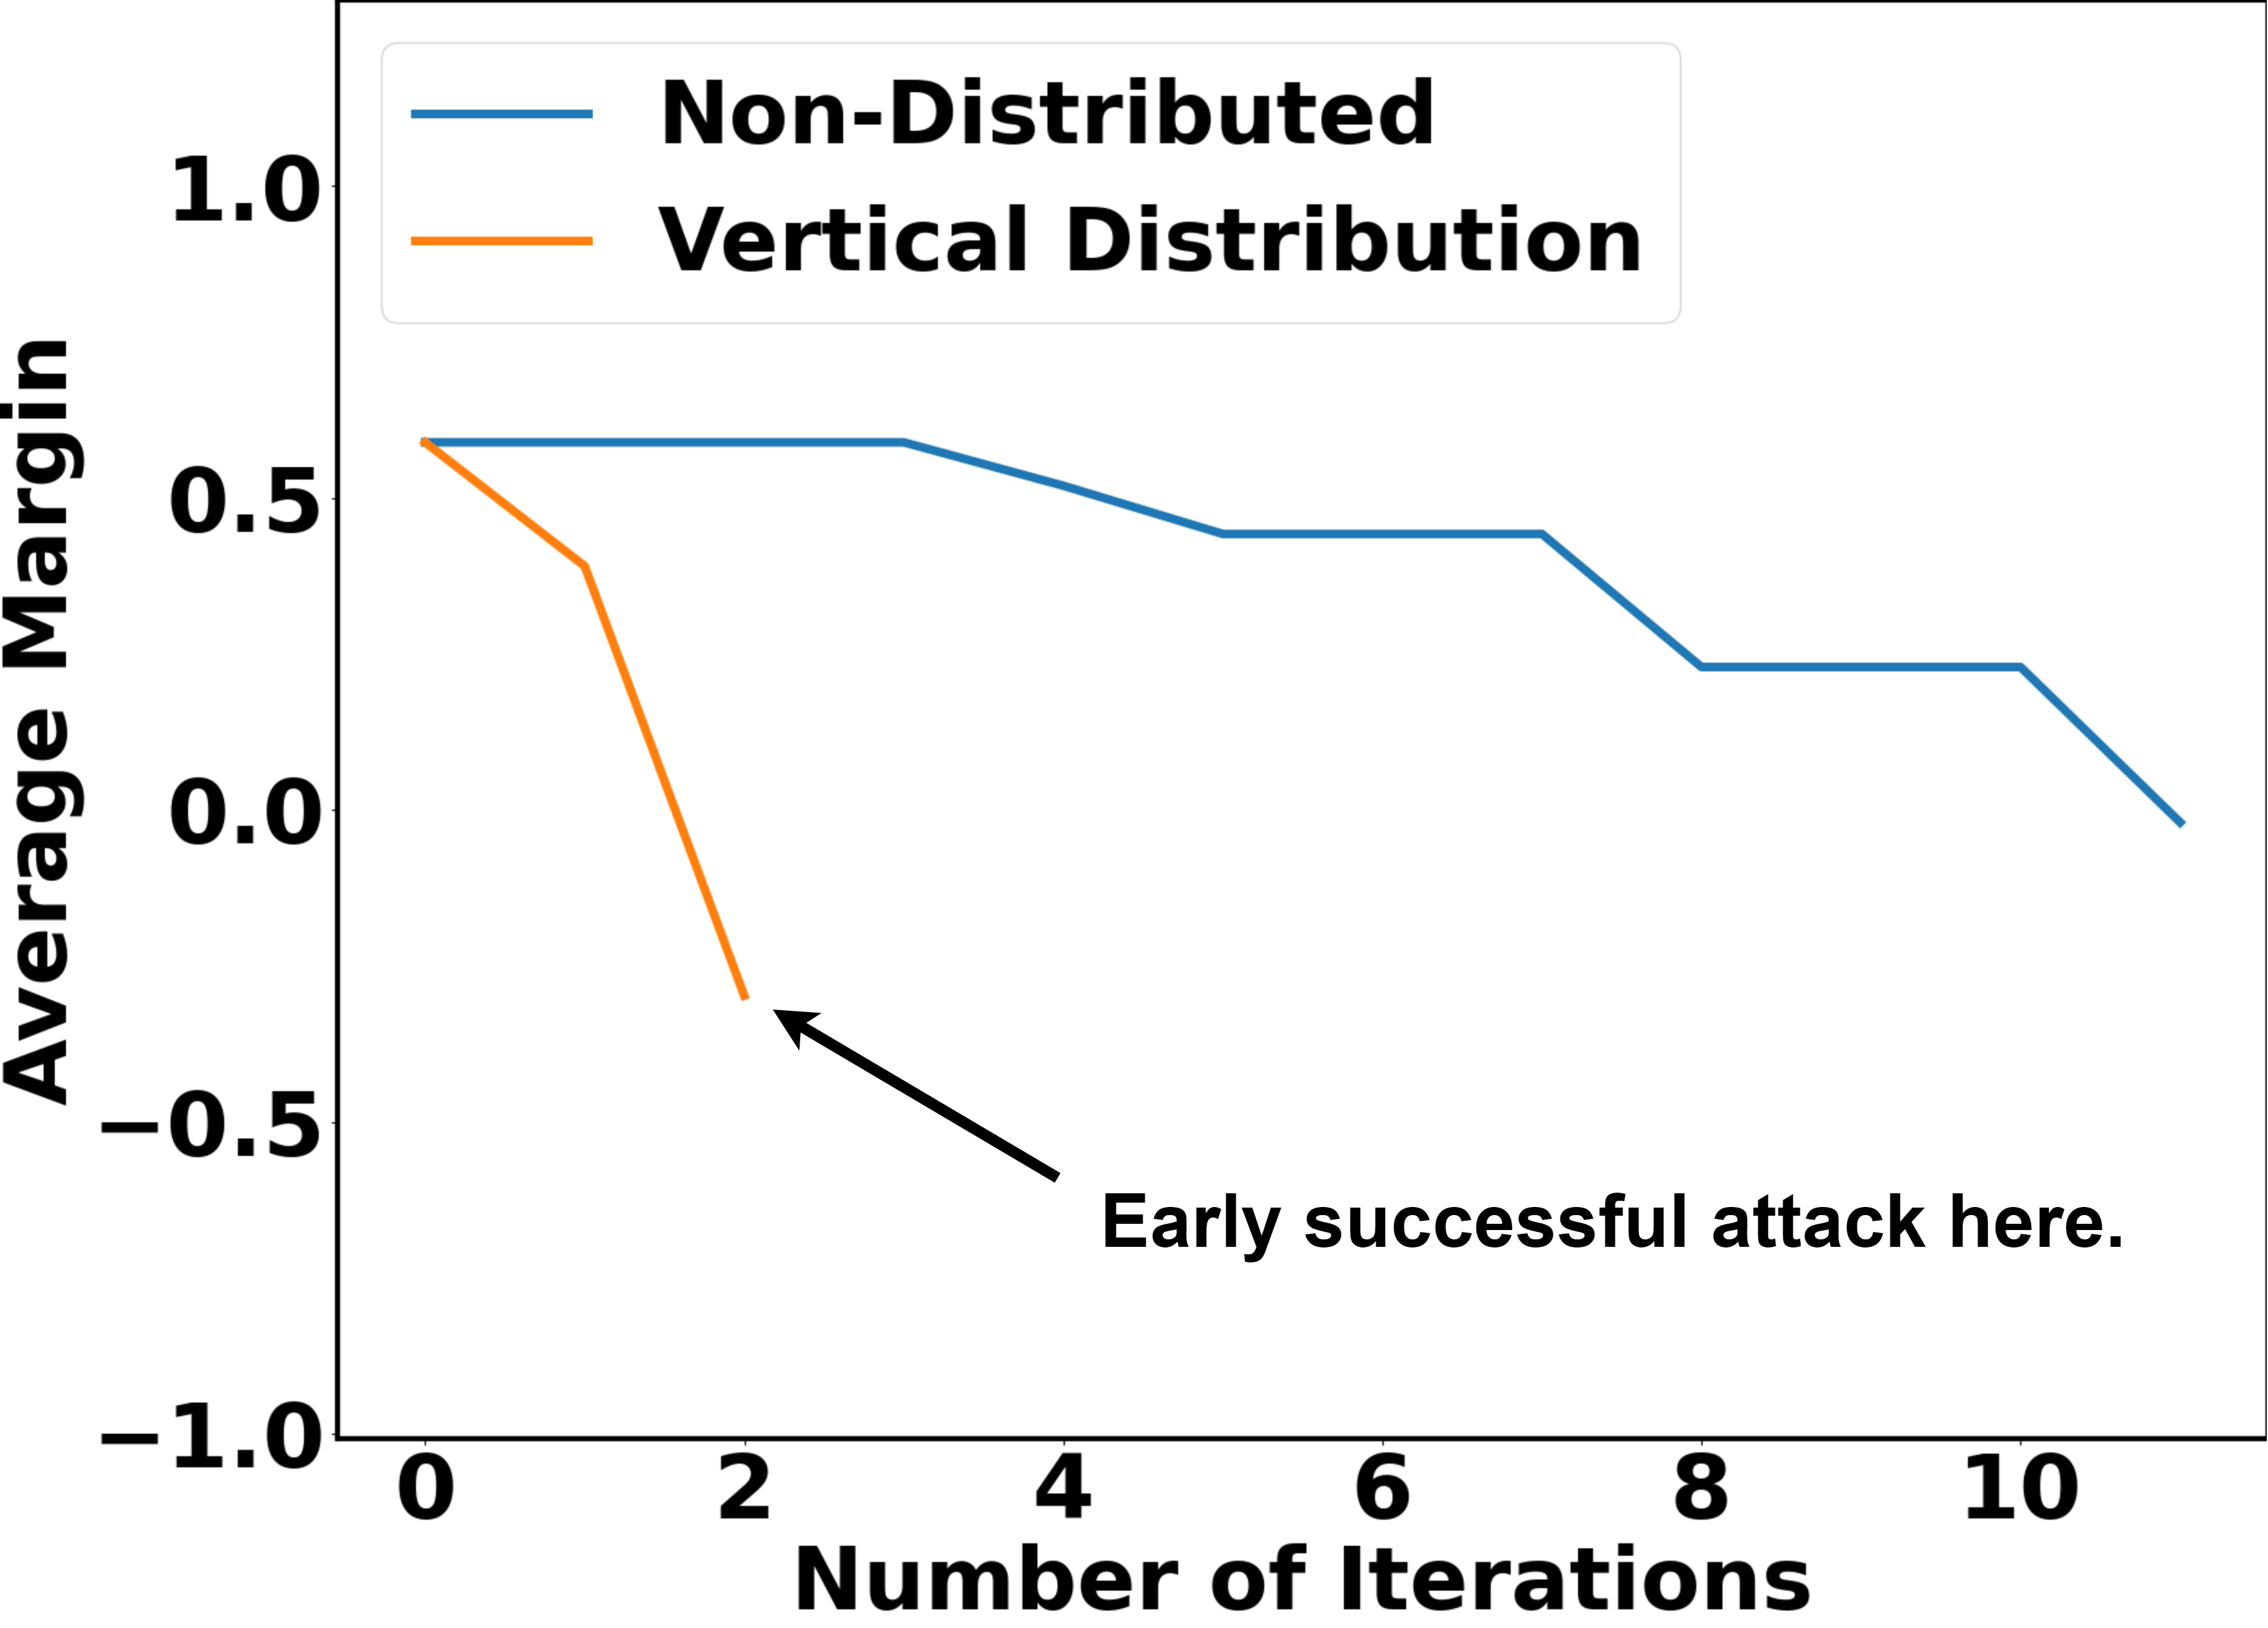
\includegraphics[width=\textwidth]{figures/chapter_classification/square_attack_vertical_margin.png}
    \caption{Square Attack}
    \label{fig:square_plot}
\end{subfigure}
\hfill
\begin{subfigure}[b]{0.32\textwidth}
    \centering
    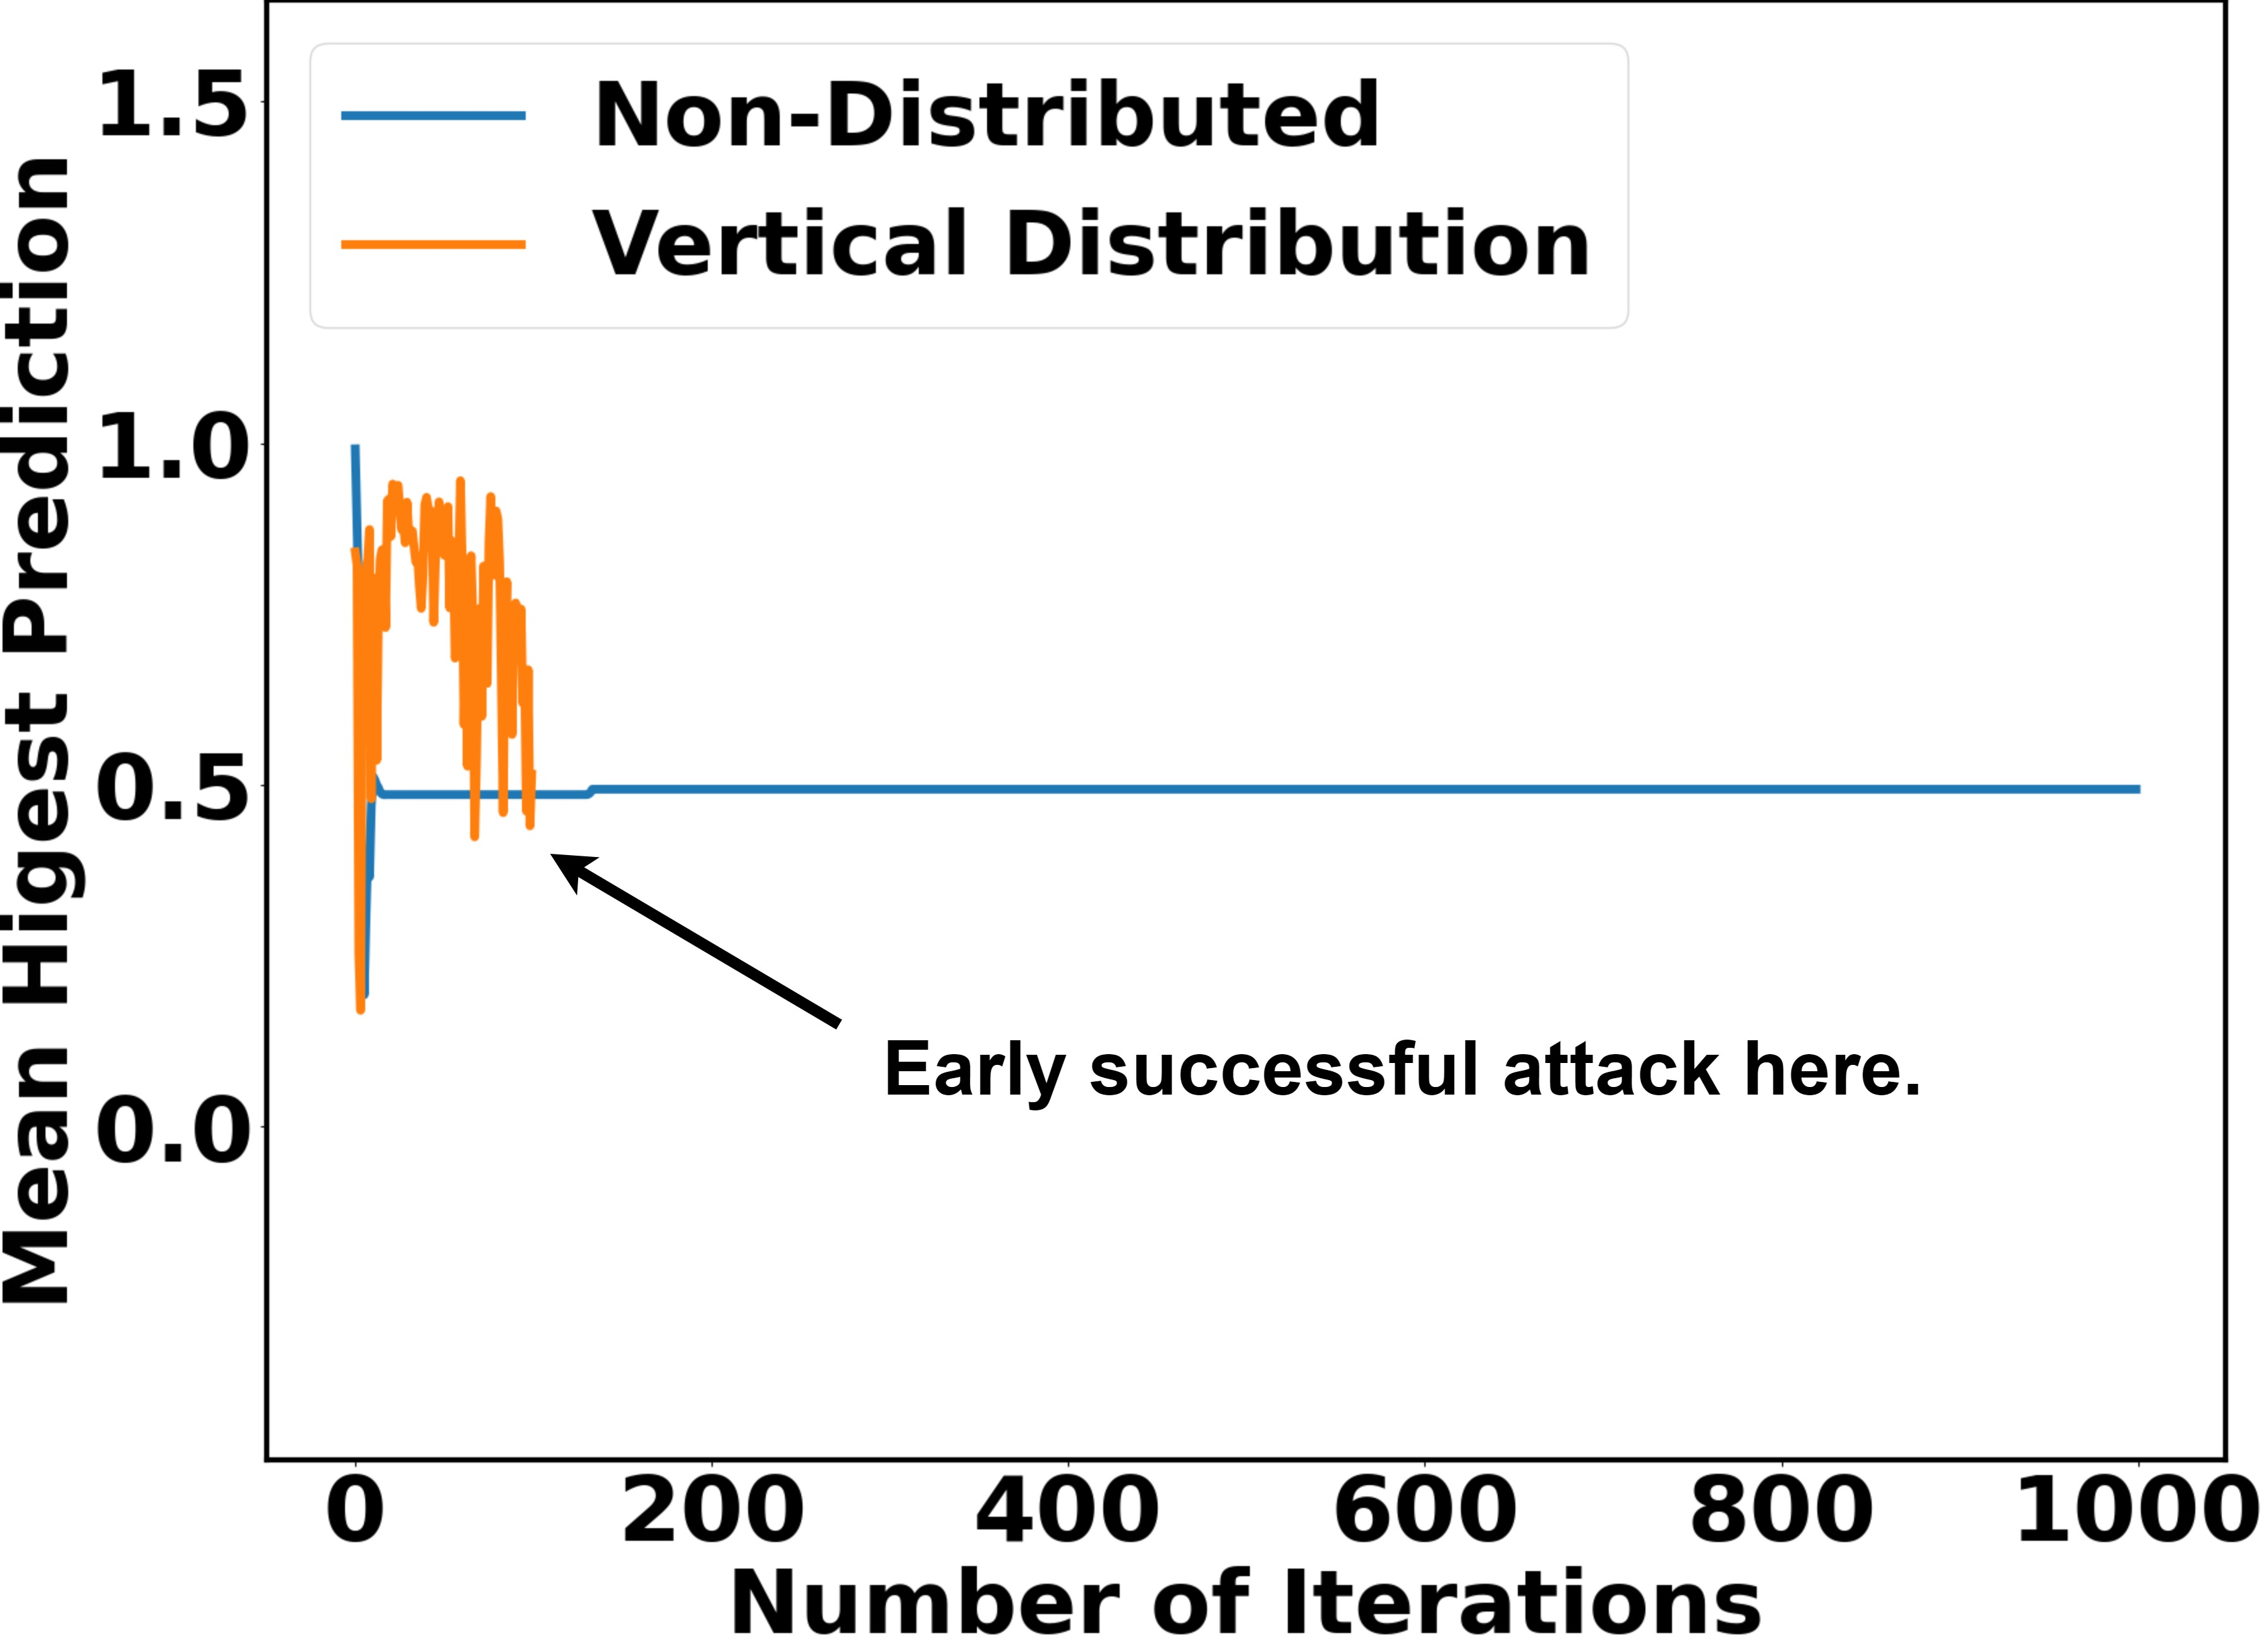
\includegraphics[width=\textwidth]{figures/chapter_classification/bandits_attack_vertical_margin.png}
    \caption{Bandits Attack}
    \label{fig:bandits_plot}
\end{subfigure}
\caption{The iteration process of different black-box attacks.}
\label{fig.vertical_plot}
\end{figure*}

% \pagebreak

\section{Conclusion}


Our research presents a novel approach to accelerating black-box attacks against online cloud services by exploiting load balancing. We introduce two general frameworks, horizontal and vertical distribution, that can be applied to existing black-box attacks to significantly reduce the total attack time. To validate the efficiency of the frameworks, we conduct experiments using three commonly used image classifiers and three commonly used black-box attacks.

Additionally, we contribute to the research community by open-sourcing our image classification cloud service, DeepAPI. This will enable future research on distributed black-box attacks and provide insights into the practical threats posed by adversarial attacks against machine learning models deployed on cloud servers.

% Our research demonstrates that it is possible to exploit load balancing to accelerate black-box attacks against online cloud services. We design two general frameworks, horizontal and vertical distribution, that can be applied to existing black-box attacks to reduce the total attack time. The efficiency of the frameworks was validated using experiments involving three commonly used image classifiers and three commonly used black-box attacks. In addition, we open-source our image classification cloud service, DeepAPI. This will facilitate future research on distributed black-box attacks and on whether adversarial attacks are a practical threat against machine learning models deployed on cloud servers.

% \clearpage

\section{The Black-box Adversarial Toolbox (BAT)}
\label{sec:bat}

We integrate distributed black-box attack methods into the Black-box Adversarial Toolbox (BAT). The objective is to achieve practical black-box attacks within limited queries and time.

\begin{figure}[H]
\centering
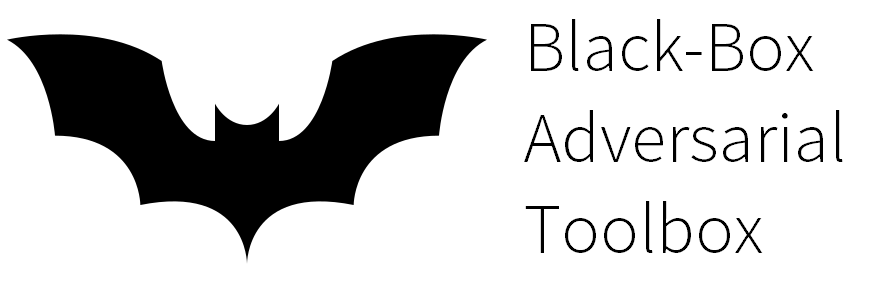
\includegraphics[scale=0.35]{figures/chapter_classification/bat.png}
\caption{The Black-box Adversarial Toolbox}
\label{fig.bat}
\end{figure}

Our demo application demonstrates that the original SimBA attack against a tiny VGG16 model pre-trained on the Cifar10 dataset takes around 200 seconds to achieve one successful attack. While the distributed SimBA attack takes only 40 seconds, which is five times faster. The acceleration ratio could grow even more as the number of nodes increases.

\begin{figure}[H]
\centering
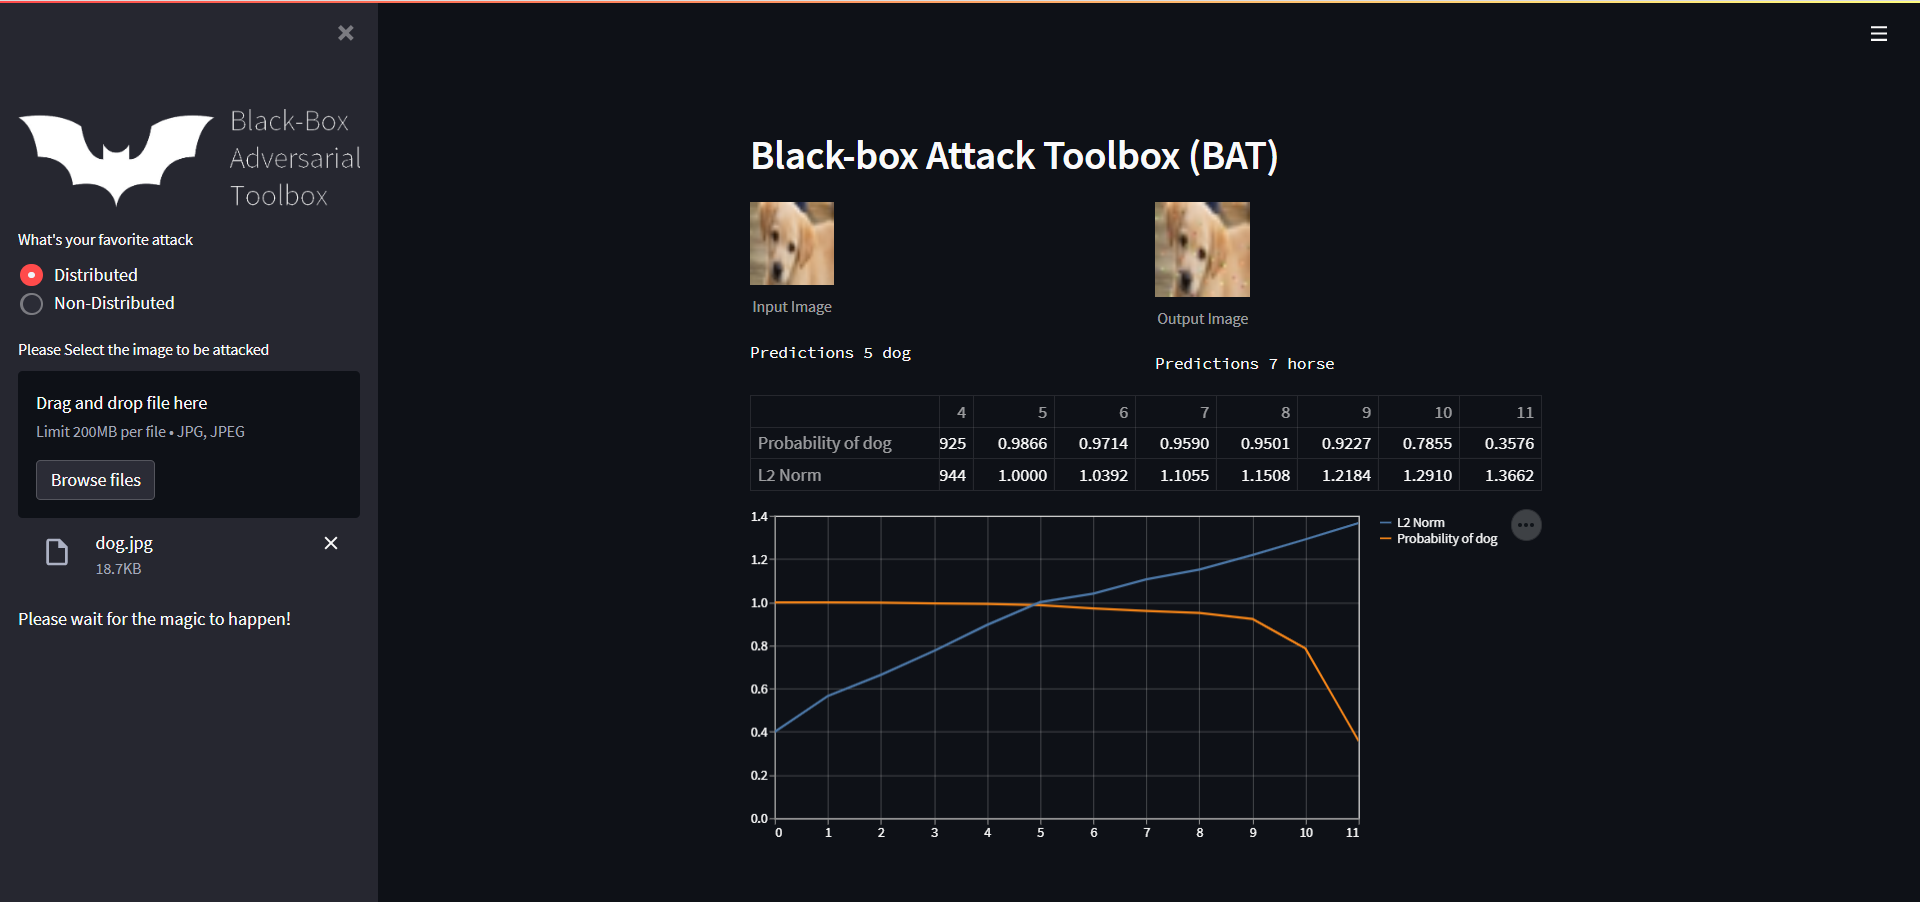
\includegraphics[width=0.75\textwidth]{figures/chapter_classification/bat_app.png}
\caption{Demon application of the Black-box Adversarial Toolbox}
\label{fig.bat_app}
\end{figure}

\clearpage

% \printbibliography[
%   keyword={chapter_classification}, heading=subbibintoc, resetnumbers=true
% ]